\documentclass{article}
\usepackage[utf8]{inputenc}
\usepackage[T1]{fontenc}
\usepackage{tgtermes}
\usepackage{mathptmx}  
\usepackage[scaled=.92]{helvet}
\usepackage{amsthm,amsmath,amssymb}
\usepackage{mathrsfs}
\usepackage[round]{natbib}  
\usepackage[colorlinks,citecolor=blue,urlcolor=blue]{hyperref}  %%check
\usepackage[dvipsnames]{xcolor}
%%%Algorithms
\usepackage[noend]{algpseudocode}
\usepackage{algorithm,amsmath}
\usepackage{mathtools}
\usepackage{newtxtext,newtxmath}
\usepackage[tight,footnotesize]{subfigure}
\usepackage[colorinlistoftodos]{todonotes}
\newcommand*{\R}{\mathbb{R}}
\newcommand*{\G}{\mathcal{G}}
\newcommand*{\Po}{\text{Prox}}
\newcommand*{\Am}{\text{argmin}}
\newcommand*{\E}{\mathbb{E}}
\newcommand*{\VRG}{\,\tilde{\nabla}_k^s}
\newcommand{\norm}[1]{\left\lVert#1\right\rVert}
\newcommand{\abs}[1]{\left|#1\right|}
\newcommand{\Iprod}[2]{\left\langle #1,#2\right\rangle}
\newcommand\myeq[2]{\mathrel{\stackrel{\makebox[0pt]{\mbox{#1}}}{#2}}}

\renewcommand{\algorithmicrequire}{
\textbf{Input:}}
\renewcommand{\algorithmicensure}{\textbf{Output:}}
\newcommand{\Initialize}{\textbf{Initialize:}{\,}}
\newcommand{\Input}{\textbf{Input:}{\,}}
\newcommand{\Output}{\textbf{Output:}{\,}}


\newtheorem{theorem}{Theorem}[section]
\newtheorem{lemma}[theorem]{Lemma}
\newtheorem{conjecture}[theorem]{Conjecture}
\newtheorem{condition}[theorem]{Condition}
\newtheorem{claim}[theorem]{Claim}
\newtheorem{question}[theorem]{Question}
\newtheorem{corollary}[theorem]{Corollary} 
\theoremstyle{definition}
\newtheorem{definition}[theorem]{Definition}
\newtheorem{statement}[theorem]{Statement}
\newtheorem{notation}[theorem]{Notation} 
\theoremstyle{remark}
\newtheorem{remark}[theorem]{Remark}
\newtheorem{assumption}[theorem]{Assumption}
\allowdisplaybreaks

\title{An Efficient Derivative-Free Proximal Stochastic Gradient Method for Nonconvex Nonsmooth Optimization}
\date{March 2018}

\begin{document}

\maketitle
\begin{abstract}
Proximal gradient method has an important role
in solving nonsmooth composite optimization problems. However, in some machine learning problems  proximal gradient method could not be leveraged because the explicit gradients of these problems are not accessible. Associated with black-box models, these  types  of  problems fall  into  zeroth-order (ZO) optimization. Several varieties of proximal zeroth-order variance reduced stochastic algorithms  for nonconvex optimization have recently been introduced  based on the first-order techniques of stochastic variance reduction. 
However, all existing zeroth-order SVRG-type  algorithms suffer from function query complexities up  to a small-degree  polynomial  of  the  problem  size. To fill this gap, we analyze a new zeroth-order stochastic gradient algorithms for optimizing nonconvex, nonsmooth finite-sum problems, called ZO-PSVRG+. The analysis of ZO-PSVRG+ recovers several
existing convergence results and improves theirs ZO oracle calls and proximal oracle calls. In particular, ZO-PSVRG+ yields simpler analysis  for a wide range of minibatch sizes, while the improvement of ZO-SVRG in \cite{ji2019improved} is only achieved for large minibatch sizes based on an involved parameter selection. We further prove ZO-PSVRG+ under Polyak-Łojasiewicz condition in contrast to existent ZO-SVRG type methods obtains a global linear convergence for a wide range of minibatch sizes. Our empirical experiments on black-box binary classification and black-box adversarial attack problem
validate  that  the studied algorithms under our new analysis  can  achieve  superior performance with a lower  query complexity. 
\end{abstract}

\section{Introduction}
\subsection{what we want to do}
In this paper, we consider the nonsmooth nonconvex optimization problems of the following form
\begin{equation}\label{problem}
\min_{x\in\R^d} F(x) =  f(x) + h(x),\,\,\,f(x):=\frac{1}{n}\sum_{i=1}^n f_i(x)
\end{equation}
where each $f_i(x)$ is possibly nonconvex and smooth function, and $h(x)$ is a nonsmooth convex function such as $l_1$-norm regularizer. 
The general structure \eqref{problem} covers
numerous machine learning areas, ranged from neural networks to  generalized linear models  
 and from convex problems like  SVM  and Lasso to highly nonconvex optimization including minimizing loss function for deep learning. We will investigate and explore a set of accelerated variance reduced stochastic zeroth-order (SZO) optimization algorithms for \eqref{problem}. Stochastic variance reduced gradient
(SVRG) is a generic and powerful methodology to decrease the variance induced by stochastic sampling \cite{johnson2013accelerating,reddi2016stochastic,nitanda2016accelerated,allen2016improved,lei2017non}. As a result of reduction in variance, it enhances the rate of convergence for stochastic gradient descent (SGD) complexity by a factor of $O(1/{\epsilon})$. To reduce the variance in SZO optimization, one may apply the comparable concepts and similar ideas in the first-order methods. 
\subsection{Background in research}
In recent years, there has been thorough studies for convex problems of the form \eqref{problem} (see e.g., \cite{nesterov2013gradient}, \cite{xiao2014proximal,defazio2014saga,lan2017optimal,allen2017katyusha}. 
In particular, in \cite{beck2009fast} a fast-converging class of proximal gradient (PG) schemes for problems with convex structure based on Nesterov's momentum acceleration are designed.  
\cite{xiao2014proximal} developed an algorithm called Prox-SVRG for large-scale problems, which
obtains a linear rate of convergence when each  $f_i$ is strongly-convex. Several stochastic PG methods were developed in \cite{bertsekas2011incremental,xiao2014proximal}  to deal with the large-scale convex problems. Because of growing applications of deep neural networks, recently the studies for nonconvex case have been noticeably growing. Nevertheless, for the generic nonsmooth nonconvex problems, the analysis is still rather sparse.  \cite{li2015accelerated} introduced a set of fast-converging PG algorithms for nonconvex structure problems. Similarly, \cite{ghadimi2016accelerated,reddi2016proximal} studied stochastic PG methods for nonconvex optimization.
Recently, \cite{li2018simple} designed an algorithm by extending the results from \cite{reddi2016proximal}, leading to an improved iteration complexity for stochastic gradient method. 
\subsection{Reason to use zeroth--order techniques}
The major adversity for these accelerated method is their designs on involving first-order information. Nevertheless , there are circumstances where the first-order gradient evaluations are computationally unrealizable, costly, or unachievable, while zeroth-order information (function information) are accessible. For instance, in online auctions and advertisement
selections, only zeroth-order information in the form of responses to the queries is accessible \cite{wibisono2012finite}. Similarly, in predictions with stochastic structure, computing the derivatives is possibly complicated or prohibited to perform, while the functional estimations of foreseen frameworks are achievable  \cite{sokolov2016stochastic}. 
For instance, in bandit \cite{shamir2017optimal} and black-box intelligence \cite{chen2017zoo} settings, only the loss function evaluations are accessible as the derivatives cannot be calculated directly. 
Thus, the derivative-free  optimization algorithm \cite{nesterov2017random} is a viable option to tackle these issues. This procedure approximates the full gradient via gradient evaluator based on only the function estimations which end up in derivative-free optimization \cite{brent2013algorithms,spall2005introduction}. 
We describe the minimization problem \eqref{problem} in this particular setting as stochastic proximal zeroth-order optimization.
Recently, zeroth-order optimization has attracted significant attention due to its diverse applications, e.g., black-box adversarial attacks on deep neural networks (DNNs) \cite{kurakin2016adversarial,papernot2017practical, chen2017zoo}, reinforcement learning \cite{choromanski2018structured} and structured prediction \cite{taskar2005learning}.
Further applications cover time-varying constrained networks with restricted computation capacity \cite{chen2019bandit,liu2017zeroth}, and model inference with black-box setting \cite{fu2002optimization,lian2016comprehensive}. 

\subsection{Problem with existing methods}
While a great number of SZO algorithms have recently been explored and studied \cite{liu2017zeroth,flaxman2005online,shamir2013complexity,agarwal2010optimal,nesterov2017random,duchi2015optimal,shamir2017optimal,dvurechensky2018accelerated,wang2017stochastic}, they are mostly employed for problems with convex structure, which confines their applications in the broad span of nonconvex problems.

 Furthermore, these methods  regularly degrade due to the large variances of SZO gradient evaluations, and consecutively, decaying rate of convergence. Hence, a practical method to obtain faster convergence for SZO is by exploiting variance reduced techniques.
Recently, various SZO variance
reduced methods have been investigated to additionally enhance the rate of convergence of ZO-SGD \cite{liu2018stochastic,liu2018zeroth}. These methods are primarily derived from SVRG algorithm, which substitutes the gradient in
SVRG \cite{johnson2013accelerating} by zeroth-order gradient
approximations. Specifically, \cite{liu2018zeroth} introduced several
zeroth-order methods, based on SVRG-type algorithms. 
 
Currently, there are only a few number of zeroth-order stochastic methods
for solving problem \eqref{problem}, e.g., \cite{ghadimi2016accelerated} and \cite{huang2019faster}. In particular, in \cite{ghadimi2016accelerated} a zeroth-order proximal stochastic gradient method has been analyzed. Nevertheless, as a result of the high variance of zeroth-order gradient approximation based on random sampling and vector sampling for two point derivative calculations, the iteration complexity of RSPGE ($O(\frac{d}{\epsilon^2})$) is notably worse than the best known rate $O(\frac{d}{{\epsilon}})$ for zeroth-order stochastic optimization. A major issue in the advancement of SZO algorithms for solving  \eqref{problem} is the order of the required number of function queries, namely SZO calls or iteration complexity. While the present zeroth-order based upon SVRG algorithms have higher convergence rate, the complexity of their function calls are all greater than each of ZO-GD and ZO-SGD. They also rely on a very small and some often diminishing stepsize of $O(\frac{1}{d})$. To perform an elaborated analysis, the term related to the dimension of the problem in the convergence studies (i.e., $d$) is a key factor with high impact on the efficiency of SZO optimization. \cite{ji2019improved} refined the ZO estimations to achieve an improved ZO complexity and enhanced convergence rate. However, their improved analysis is only for smooth functions based on a complicated parameter selection and it is only valid for large minibatch sizes.
We design an accelerated ZO proximal variants by applying variance reduced gradient approximation for nonsmooth composite optimization. This provides a lower iteration complexity towards $O(1/\epsilon )$, which is to our knowledge the best iteration complexity bound obtained thus far for proximal ZO stochastic optimization with nonconvex structure.
This demonstrates an improvement for ZO iteration complexity up to a factor of ${d}$.

\subsection{Compare with other methods}
We compared the results from our analysis and other comparable SZO algorithms in Table \ref{table-compare}. It \ref{table-compare} indicates
that RGF has the largest query complexity and yet has the worst convergence rate. ZO-SVRG-coord
and ZO-ProxSVRG/SAGA provide an improved rate of convergence $O(d/\epsilon )$ due to using variance reduction techniques. On the other hand, existing SVRG type zeroth-order algorithms are affected by worse function query complexities compared with RSPGF, while ZO-PSVRG+ could achieve better trade-offs between the convergence rate and the query complexity.


\section{Main Challenge}
Despite the fact that proximal SVRG has indicated a huge promise for first-order algorithms, utilizing identical concepts to ZO optimization is not effortless. 
Due to the perturbation induced by ZO gradient estimation, SZO algorithms have complex joint structures, which make their analysis difficult in many settings. The other major difficulty is due to the fact that that ProxSVRG is based upon the notion that stochastic gradient is an unbiased approximation of the actual full gradient, which is not retained in the ZO case. Thus, it is a challenging question if the proximal ZO stochastic variance reduced gradient could accelerate the convergence of proximal ZO algorithms with arbitrary minibatch sizes. In this paper, we plan to address this question and in particular fill the void between
SZO optimization and ProxSVRG by improving the complexity of exiting ZO variance reduced methods for problem \eqref{problem}.



\section{Main contributions}
We present a novel analysis for an existing ZO-SVRG-Coord algorithm introduced in \cite{liu2018zeroth,ji2019improved}, and
prove that ZO-PSVRG+ based on  our new analysis surpasses other state-of-the-art SVRG-type zeroth-order methods as well as RSPGF.
We concentrate on several important debatable questions in these methods. To be specific, we somewhat address the open question if the dependence on the dimension $d$ for the convergence analysis proposed in \cite{liu2018zeroth} is optimal. Our work provides an inclusive analysis on how ZO gradient approximation influence ProxSVRG on both  convergence rate and function query complexity. This
is performed based on the novel structure of recently introduced SZO algorithms.
Note that problem \eqref{problem} does not necessarily satisfy bounded gradient assumption in \cite{ghadimi2016accelerated,huang2019faster}.
We prove that compared to
ProxSVRG, ZO-PSVRG+ obtains a sublinear convergence with SZO complexity of $O(1/\epsilon)$.
The convergence results are declared with respect to the number of stochastic zeroth-order (SZO) queries and proximal oracle (PO) calls. 
Based on our new analysis, we summarize the following results from this parer:

1) Our analysis yields iteration complexity $O(\frac{1}{{\epsilon}})$ corresponding to $O(\frac{d}{\epsilon^2})$ of RSPGF \cite{ghadimi2016accelerated}  and $O(\frac{d}{\epsilon})$ of ZO-ProxSVRG/SAGA  \cite{huang2019faster} (the existing variance-reduce SZO proximal algorithm for solving nonconvex nonsmooth problems).  
Thus, our results have better or no dependence on
$d$ in contrast to the existing proximal variance-reduced SZO methods. Note that the number of PO calls equal to $O(1/\epsilon)$  and $O(1/\epsilon^2)$ for ZO-PSVRG+ and RSPGF, respectively.  ZO-PSVRG+ also matches the best result achieved by ZO-SVRG-Coord-Rand with $b = d n^{2/3}$ for $m = n^{1/3}$ in \cite{ji2019improved}, while our results are valid for any minibatch sizes as detailed in the following sections.  
Indeed, since generally  in training model parameters intermediate minibatch sizes are preferred, it is necessary to analyze and study the convergence behavior for minibatchs of moderate or single sizes.


2) The convergence analysis for ZO-PSVRG+ is not complicated in contrast to  ZO-SVRG-Coord in \cite{liu2018zeroth,ji2019improved}, and yields simpler proofs. Our analysis achieves new iteration complexity bounds and improves the effectiveness of  all the existing ZO-SVRG-based algorithms in addition to RSPGF for nonconvex nonsmooth composite optimization, which is the best results to our latest knowledge (see Table \ref{table-compare}). 


3) For the nonconvex functions under Polyak-Łojasiewicz condition \cite{polyak1963gradient}, we show that ZO-PSVRG+
obtains a global linear rate of convergence  equivalent to first-order ProxSVRG. Thus, ZO-PSVRG+ can certainly achieve linear convergence in some zones without restarting. To the best of
our knowledge, this is the first paper that leverages the PL condition for improving the convergence of of ZO-ProxSVRG for problem \eqref{problem} with arbitrary minibatch size. It is also noticeable that the convergence rate obtained in this exploration is comparable to the first-order ProxSVRG. This generalizes the results of \cite{duchi2015optimal} and  achieves linear convergence compared to the sublinear convergence rate in their paper.
In \cite{ji2019improved}, the authors show that  ZO-SPIDER-Coord achieves linear convergence under PL condition and with $b = O(n^{1/2})$.  
note that due to both computational and statistical efficiency, convergence analysis for practical minibatch sizes is demanding. Also see the remarks after Theorem \ref{zo-pl-cond} for more details. 

Finally, to demonstrate the efficiency and adaptability of our approach to achieve a balance between the rate of convergence and the number of SZO queries, we perform some
experimental evaluations for two distinct applications: black-box binary classification and universal adversarial
attacks on black-box deep neural network models. The empirical results and
theoretical investigations verify the effectiveness of our algorithms.


\section{Related Works}
Derivative-free (zeroth-order) methods have been efficiently utilized for solving numerous machine learning problems when the computation of the true gradient is infeasible. In ZO algorithms, a full gradient is generally estimated based on either a one-point or a two-point gradient approximation. The one-point estimator obtains a gradient estimate $\hat{\nabla} f(x)$ by probing $f$ at a single random point near to $x$ \cite{flaxman2005online,shamir2013complexity},  while the two-point estimator computes a difference of two random function probings \cite{agarwal2010optimal,nesterov2017random}. In this paper, we concentrate on the two-point gradient approximation since it has a lower variance and thus amends the iteration complexity of ZO algorithms. \cite{nesterov2017random} proposed several stochastic derivative-free
algorithms by employing Gaussian smoothing method.  A zeroth-order mirror descent algorithm is analyzed in \cite{duchi2015optimal}. 
More recently, \cite{yu2018generic,dvurechensky2018accelerated} introduced some accelerated zeroth-order algorithms for convex optimization. The recent studies confirmed that ZO algorithms typically agree with the complexity of first-order algorithms up to a small-degree polynomial of the problem size $d$.

These zeroth-order algorithms mostly target (strongly) convex problems. Despite the extensive studies for the convex structures, the studies for nonconvex ZO methods are relatively limited.  Essentially, there are many nonconvex machine learning application, where the explicit derivatives are not accessible, e.g., nonconvex black-box learning problems \cite{chen2017zoo,liu2018zeroth}. Thus, developing zeroth-order stochastic methods for the nonconvex optimization is indeed demanding.
\cite{ghadimi2013stochastic} and \cite{nesterov2011random} proposed ZO-GD and
its corresponding stochastic algorithm ZO-SGD, respectively. \cite{liu2018stochastic} introduced a variance reduced stochastic zeroth-order method with  Gaussian smoothing. More recently, \cite{liu2018zeroth} presented a thorough analysis based on SVRG algorithms. \cite{ji2019improved} elaborated the results in \cite{liu2018zeroth} and achieved improved bounds based on a complicated parameter selection, however their improvements relies on large minibatch sizes. 
Recently, for nonsmooth nonconvex problems \cite{huang2019faster} provided two algorithms called ZO-ProxSVRG and ZO-ProxSAGA, which are based on the well-known variance reduction techniques ProxSVRG and ProxSAGA \cite{reddi2016proximal}. Before that,  \cite{ghadimi2016accelerated} also considered the stochastic case (here we denote
it as RSPGF). However, RSPGF requires increasing or large minibatch sizes i.e., $\Omega(1/\epsilon)$. Note that due to the
growing minibatch sizes, RSPGF may change to deterministic proximal gradient descent (ZO-ProxGD) after few iterations. Further, \cite{liu2018stochastic} have also analyzed a zeroth-order algorithm for solving nonconvex nonsmooth problems, which are different from problem \eqref{problem}.
In order to deal with the large-scale problems, several asynchronous stochastic zeroth-order algorithms have been studied, e.g., \cite{gu2018inexact,lian2016comprehensive,gu2018faster}.
In \cite{lian2016comprehensive}, an asynchronous ZO stochastic coordinate
descent (ZO-SCD) was designed with a convergence rate of $O(d/\epsilon^2)$.
The convergence rate of asynchronous SZO further improved in \cite{gu2018faster} 
 by integrating SVRG techniques with stochastic coordinate descent method.
  
Even though the abovementioned zeroth-order stochastic algorithms can effectively solve the problems with nonconvex structure, there are limited number of zeroth-order stochastic methods for nonconvex nonsmooth composite problems. We emphasize that, in contrast to existing ZO proximal methods, our analysis do not require bounded gradient assumption, which is not valid for many unconstrained optimization problems. 
It should be highlighted that computing full-gradient may not be effective for large-scale machine learning problems. Thus, we focus on studying a more general framework of ZO-ProxSVRG with different gradient estimators.
\begin{table}\label{table-compare}
\begin{center}
\begin{tabular}{ |l|l|l|l|l| } 
 \hline
 Method & Problem & Stepsize& Convergence rate & SZO complexity\\ 
 \hline
  
 RGF (\cite{nesterov2017random}) & NS(C) & $O\left(\frac{1}{\sqrt{dT}}\right)$ & $O\left(\frac{d^2}{\epsilon^2}\right)$ &$O\left(\frac{nd^2}{\epsilon^2}b\right)$\\
 RSPGF (\cite{ghadimi2016accelerated}) & S(NC)+NS(C) & $O\left(1\right)$ & $O\left(\frac{d}{\epsilon^2}\right)$ &$O\left(\frac{nd}{\epsilon^2}\right)$\\ 
 ZO-SVRG-Coord (\cite{liu2018zeroth}) & S(NC)& $O\left(\frac{1}{{d}}\right)$ & $O\left(\frac{d}{\epsilon}\right)$ & $O(\frac{nd^2}{\epsilon}+\frac{d^2b}{\epsilon})$\\
 ZO-SVRG-Coord-Rand (\cite{ji2019improved}) & S(NC)& $O\left(\frac{1}{{dn^{2/3}}}\right)$ & $O\left(\frac{dn^{2/3}}{\epsilon}\right)$ & $O(\min\{\frac{dn^{2/3}}{\epsilon},\frac{d}{\epsilon^{5/3}}\})$\\
  ZO-ProxSVRG-Coord (\cite{gu2018faster}) & S(NC)+NS(C) & $O\left(\frac{1}{{d}}\right)$ & $O\left(\frac{d}{\epsilon}\right)$ & $O(\frac{nd^2}{\epsilon\sqrt{b}}+\frac{md^2\sqrt{b}}{\epsilon})$\\
   ZO-ProxSAGA-Coord (\cite{gu2018faster}) & S(NC)+NS(C)& $O\left(\frac{1}{{d}}\right)$ & $O\left(\frac{d}{\epsilon}\right)$ & $O(\frac{nd^2}{\epsilon\sqrt{b}})$\\
   ZO-PSVRG+ (CoordSGE) (Ours)  & S(NC)+NS(C) & $O\left(1\right)$ & $O\left(\frac{1}{\epsilon}\right)$ & $O\left(s_n\frac{d}{\epsilon \sqrt{b}}+\frac{bd}{\epsilon}\right)$\\
   ZO-PSVRG+ (RandSGE) (Ours)  & S(NC)+NS(C) & $O\left(\frac{1}{\sqrt{d}}\right)$ & $O\left(\frac{\sqrt{d}}{\epsilon}\right)$ & $O\left(s_n\frac{d\sqrt{d}}{\epsilon \sqrt{b}}+\frac{b\sqrt{d}}{\epsilon}\right)$\\
   ZO-PSVRG+ (CoordSGE) (Ours) & S(PL)+NS(C) & $O\left(1\right)$ & $O\left(\log(\frac{1}{\epsilon})\right)$ & {\scriptsize$O(s_n \frac{d}{\lambda\sqrt{\gamma} m}\log\frac{1}{\epsilon}+\frac{bd}{\lambda\sqrt{\gamma}}\log\frac{1}{\epsilon})$}\\
   ZO-PSVRG+ (RandSGE) (Ours) & S(PL)+NS(C) & $O\left(\frac{1}{\sqrt{d}}\right)$ & $O\left(\sqrt{d}\log(\frac{1}{\epsilon})\right)$ & {\scriptsize$O(s_n\frac{d\sqrt{d}}{\lambda\sqrt{\gamma} m}\log\frac{1}{\epsilon}+\frac{b\sqrt{d}}{\lambda\sqrt{\gamma}}\log\frac{1}{\epsilon})$}\\
 \hline
\end{tabular}\caption{Summary of convergence rate and function query complexity of SZO algorithms. S: Smooth, NS: Nonsmooth, NC: Nonconvex, C: Convex, SC: Strong Convexity, and PL: Polyak-Łojasiewicz Condition. $s_n = \min\{n, \frac{1}{\epsilon}\}$}.
\end{center}
\end{table}

\section{Preliminary}
In the following we specify and illustrate some details on ZO gradient approximations.
Considering a single loss function $f_i$, a two-point random stochastic gradient estimator (RandSGE) $\hat{\nabla}_r f_i(x)$ is defined as \cite{nesterov2017random,gao2018information}
\begin{equation}\label{gradestrand}
\hat{\nabla}_r f_i(x, u_i) = \frac{d(f_i(x+\mu u_i) - f_i(x))}{\mu}u_i,\qquad i\in [n],
\end{equation}
where $d$ is the number of optimization variables, $\{u_i\}$ are i.i.d. random directions drawn from a uniform distribution over a unit sphere and $\mu > 0$ is a smoothing parameter  \cite{flaxman2005online,shamir2017optimal,gao2018information}. Typically, RandSGE is a biased estimation to the actual gradient $\nabla f_i(x)$, and its bias decreases as $\mu$ approaches zero. Nevertheless, in practice, if $\mu$ is too small, the function variation
could be signified by the noise in the system when the rate of noise to signal is high  
 \cite{lian2016comprehensive}.
To obtain a higher quality approximation for ZO gradient, one can apply coordinate gradient estimation (CoordSGE) \cite{gu2018inexact,gu2018faster,liu2018zeroth} to evaluate the gradients as shown:
\begin{equation}\label{gradestcoord}
\hat{\nabla} f_i(x) = \sum_{j=1}^d \frac{f_i(x+\mu e_j) - f_i(x-\mu e_j)}{2\mu}e_j,\qquad i\in [n],
\end{equation}
where $e_j$ is a standard basis vector with $1$ at its $j$-th coordinate and $0$ otherwise, and $\mu$ is a smoothing parameter. In contrast to RandSGE, CoordSGE is deterministic and needs $d$ times more ZO function calls. 
However, our studies reveal that for ZO variance-reduced
methods, although the coordinate-wise gradient estimator
demands more ZO calls than the two-point random gradient approximation,
it assures a more accurate ZO estimation, which results in a
larger stepsize and a speedier convergence. More details on ZO gradient estimation can be found in \cite{kazemi2018proximal}.

Since proximal gradient method requires to compute the gradient  in each iteration, it cannot be used to tackle the optimization problems where the computation of explicit gradient of function $f(x)$ is infeasible.
Based on the ZO gradient estimation \eqref{gradestcoord}, we present a zeroth-order proximal gradient descent method, which undertakes iterations of the form:
\begin{equation}
x_{t}^s= \Po_{\eta h}(x_{t-1}^s - \eta \hat{\nabla} f(x_{t-1}^s)),\qquad t=1, 2, \ldots
\end{equation}
where $\hat{\nabla} f=\frac{1}{n}\sum_{i=1}^n \hat{\nabla} f_i(x)$ and 
\begin{equation}\label{po-operator}
\Po_{\eta h}(x) := \text{arg}\,\,\min_{y\in\R^d}\left(h(y)+\frac{1}{2\eta}\norm{y-x}^2\right)
\end{equation}
In the following we assume that the
nonsmooth convex function $h(x)$ in \eqref{problem} is well-defined, i.e., the proximal operator \eqref{po-operator} can be computed effectively.
\subsection{Gradient Mapping}
For convex problems, generally the optimality gap $F(x) - F(x^*)$ is applied as the convergence metric. But for general nonconvex problems, the gradient norm is generally employed as the convergence metric. For instance, for smooth nonconvex optimization (i.e., $h(x) = 0$), \cite{ghadimi2013stochastic,reddi2016stochastic,
lei2017non,liu2018zeroth}  applied $\norm{\nabla F(x)}^2$ (i.e., $\norm{\nabla f(x)}^2$ ) as the convergence criterion. Aiming to investigate the
convergence behavior for nonsmooth nonconvex problems, it is needed to define the gradient mapping as illustrated in \cite{ghadimi2016accelerated,reddi2016proximal,huang2019faster}:
\begin{equation}
g_{\eta}(x) = \frac{1}{\eta}(x-\Po_{\eta,h}(x-\eta \nabla f(x)))
\end{equation}
If $h(x)$ is a constant function , it is noted that this gradient mapping reduces to the ordinary gradient:
$g_{\eta}(x) = \nabla F(x) = \nabla f(x)$. In this paper, we use the gradient mapping $g_{\eta}(x)$ as the convergence metric similar to
\cite{ghadimi2016accelerated,reddi2016proximal,parikh2014proximal}.
For the problems with nonconvex structure, if $g_{\eta}(x) = 0$, the point $x$ is a stationary point (Parikh, Boyd, and others, 2014). Hence, we can
exploit the following definition as the convergence metric.
\begin{definition}
The point $x$ is referred to an $\epsilon$-accurate, if $\E\norm{g_{\eta}(x)}^2 \leq \epsilon$, for some $\eta > 0$.
\end{definition}
\section{ZO Proximal Stochastic Method (ZO-PSVRG+)}
\begin{algorithm}\label{APGnonconvex-Algo}
\caption{ZO-PSVRG+}
\begin{algorithmic}[1]
\State\Input initial point $x_0$, batch size $\mathcal{B}$, minibatch size $b$, epoch length $m$, stepsize $\eta$
\State\Initialize $\tilde{x}^0 = x_0$
\For{ $s=1,2,\ldots, S$ }
\State $x_0^s = \tilde{x}^{s-1}$
\State $\hat{g}^s = \frac{1}{\mathcal{B}} \sum_{j\in I_{\mathcal{B}}} \hat{\nabla} f_j (\tilde{x}^{s-1})$
\For{ $t=1,2,\ldots, m$ }
\State Compute ${\hat{v}}_{t-1}^s$ according to \eqref{zo-grad-fo} or \eqref{zo-grad-fo-rand}
\State $x_{t}^s= \Po_{\eta h}(x_{t-1}^s - \eta \hat{v}_{t-1}^s)$
\EndFor
\State $\tilde{x}^{s} = x_m^s$
 \EndFor
 \State\Output $\hat{x}$ chosen uniformly from $\{x_{t-1}^s\}_{t\in [m], s\in [S]}$
\end{algorithmic}
\end{algorithm}
In this section, we present a proximal stochastic gradient algorithm called ZO-PSVRG+ based on variance reduced approach of ProxSVRG in \cite{xiao2014proximal,reddi2016proximal,li2018simple}.
. The description of ZO-PSVRG+ is presented in Algorithm \ref{APGnonconvex-Algo}.
Our method has two types of random sampling. In the outer iteration,
we calculate the gradient consisting of $\mathcal{B}$ samples. In the inner iteration, we randomly  choose a minibatch of samples of size $b$ to approximate the gradient.
 We call $\mathcal{B}$ and $b$  the batch and  minibatch sizes, respectively.

The major difference of our ZO-PSVRG+  and ZO-ProxSVRG is that we avoid the evaluation of the total gradient before each epoch, i.e., the number of samples $\mathcal{B}$ may not equal to $n$ (see Line 5 of Algorithm \ref{APGnonconvex-Algo}).  However, in ZO-SVRG-Coord and ZO-ProxSVRG-Coord it is assumed $\mathcal{B} = n$. If $\mathcal{B} = n$, ZO-PSVRG+ is equivalent to ZO-ProxSVRG  since Step 7 of Algorithm \ref{APGnonconvex-Algo}. Our analysis implies the results for ZO-ProxSVRG-Coord (i.e, $\mathcal{B} = n$) are novel and improve the existing analysis. In addition, ZO-PSVRG+ generalizes the existing variance-reduced methods to a more general nonsmooth nonconvex setting using a direct  analysis of zeroth-order methods and provides simpler analysis. The main idea in variance-reduced algorithms is to construct an additional sequence $\tilde{x}^{s-1}$ at which the full gradient is computed for obtaining  a revised stochastic gradient estimate
\begin{equation}\label{grad-fo}
{{v}}_{t-1}^s = \frac{1}{b} \sum_{i\in I_b}\left({\nabla} f_{i}(x_{t-1}^s)-{\nabla} f_{i}(\tilde{x}^{s-1})\right)+{g}^s
\end{equation}
where ${{v}}_{t-1}^s$ represents the gradient estimate at $x_{t-1}^s$ and  ${g}^s= \frac{1}{\mathcal{B}}\sum_{i\in I_{\mathcal{B}}}{\nabla} f_{i}(\tilde{x}^{s-1})$. The main characteristic of \eqref{grad-fo} is that ${{v}}_{t-1}^s$ is an unbiased gradient approximation of $\nabla f(x_{t-1}^s)$. In the ZO framework, the mix gradient \eqref{grad-fo} is estimated by applying only function evaluations, specified by
\begin{equation}\label{zo-grad-fo}
{\hat{v}}_{t-1}^s = \frac{1}{b} \sum_{i\in I_b}\left(\hat{\nabla} f_{i}(x_{t-1}^s)-\hat{\nabla} f_{i}(\tilde{x}^{s-1})\right)+\hat{g}^s\qquad\text{ZO-PSVRG+}
\end{equation}

or 
\begin{equation}\label{zo-grad-fo-rand}
{\hat{v}}_{t-1}^s = \frac{1}{b} \sum_{i\in I_b}\left(\hat{\nabla}_r f_{i}(x_{t-1}^s, u_i)-\hat{\nabla}_r f_{i}(\tilde{x}^{s-1}, u_i)\right)+\hat{g}^s\qquad\text{ZO-PSVRG+ (RandSGE)}
\end{equation}
where $\hat{g}^s= \frac{1}{\mathcal{B}}\sum_{i\in I_{\mathcal{B}}}\hat{\nabla} f_{i}(\tilde{x}^{s-1})$,   $\hat{\nabla} f_{i}$ is a ZO gradient approximation given by CoordSGE and $\hat{\nabla}_r f_{i}$ is a ZO gradient estimate given by RandSGE.  

Note that, $\E_{I_b}[\hat{v}_{t-1}^s] = \hat{\nabla} f(x_{t-1}^s) \neq {\nabla} f(x_{t-1}^s)$, i.e., this stochastic gradient is a biased approximation of the actual gradient.
In the other words, the unbiased assumption on gradient approximates utilized in ProxSVRG (\cite{reddi2016proximal,li2018simple}) is no longer valid. We emphasize that the biased ZO gradient estimation yields a fundamental challenge in the analyzing ZO-PSVRG+.
Hence, adjusting the similar concepts from ProxSVRG to zeroth-order algorithm \ref{APGnonconvex-Algo} is not effortless and requires an elaborated analysis of ZO-PSVRG+. To tackle this issue, we derive an upper bound for the variance of the gradient approximation $\hat{v}_t^s$ by selecting an appropriate stepsize $\eta$ and smoothing parameter $\mu$ to control
variance of gradient estimation which is discussed later.

\section{Convergence Analysis}
Now, we provide some
minimal assumptions for problem \eqref{problem} as demonstrated in the sequel:
\begin{assumption}\label{Lip-Zoo}
For $\forall i\in{1,2,\ldots,n}$, gradient of the function $f_i$ is Lipschitz continuous with a Lipschitz constant $L > 0$, such that 
\[
\norm{\nabla f_i(x) - \nabla f_i(y)}\leq L \norm{x-y},\,\,\forall x,y\in\R^d.
\]
\end{assumption}

\begin{assumption}\label{Var-Zoo}
For $\forall x\in\R^d$, $\E\left[\norm{\hat{\nabla} f_i(x) - \hat{\nabla} f(x)}^2\right] \leq \sigma^2$, where $\sigma > 0$ is a constant and $\hat{\nabla} f_i(x)$ is a CoordSGE gradient approximation of $\nabla f_i(x)$.
\end{assumption}
Both of Assumptions \ref{Lip-Zoo} and \ref{Var-Zoo} are standard assumptions applied in nonconvex optimization. The first assumption is for the convergence studies of the zeroth-order algorithms \cite{ghadimi2016accelerated,nesterov2017random,
liu2018zeroth}. The second assumption provides the bounded variance of zeroth-order gradient approximates \cite{lian2016comprehensive,liu2018stochastic,
liu2018zeroth,hajinezhad2017zeroth}. Note that due to the error estimation for CoordSGE, this assumption is equivalent to the bounded  variance of true gradients. Assumption \ref{Var-Zoo} is weaker than the assumption of bounded gradients  \cite{liu2017zeroth,hajinezhad2017zeroth},
while, we are capable to analyze more complicated problem \eqref{problem} involving a non-smooth part and obtain faster convergence rates. Assumption \ref{Var-Zoo} is essential in order to obtain a convergence result independent of $n$.
Below, We start by deriving an upper bound for the variance of estimated gradient $\hat{v}_{t-1}^s$ based on CoordSGE.
\begin{lemma}\label{var-estimate-lem}
Given the mix gradient estimation $\hat{v}_{t-1}^s = \frac{1}{b} \sum_{i\in I_b}\left(\hat{\nabla} f_{i}(x_{t-1}^s)-\hat{\nabla} f_{i}(\tilde{x}^{s-1})\right)+\hat{g}^s$ with $\hat{g}^s = \frac{1}{\mathcal{B}} \sum_{j\in I_{\mathcal{B}}} \hat{\nabla} f_j (\tilde{x}^{s-1})$, then the following inequality holds. 
\begin{equation}
\begin{split}
\E\left[\eta\norm{\nabla f(x_{t-1}^s)-{\hat{v}_{t-1}^s}}^2\right] \leq&  \frac{6\eta L^2}{b}\E\left[\norm{x_{t-1}^s-\tilde{x}^{s-1}}^2\right]\\
&+ 2\frac{I\{\mathcal{B} < n\}\eta \sigma ^2}{\mathcal{B}}+\eta \frac{7 L^2 d^2 \mu^2}{2}
\end{split}
\end{equation}
\end{lemma}
\begin{proof}
We have
\begin{align}
  \E&\left[\eta\norm{\nabla f(x_{t-1}^s)-{\hat{v}_{t-1}^s}}^2\right]\notag\\
   =&\E\left[\eta\norm{\frac{1}{b}\sum_{i\in I_b}\left(\hat{\nabla} f_i(x_{t-1}^s)-\hat{\nabla} f_i(\tilde{x}^{s-1})\right) - \left(\nabla f(x_{t-1}^s)-\hat{g}^s\right)}^2\right]\notag\\
   =&\E\left[\eta\norm{\frac{1}{b}\sum_{i\in I_b}\left(\hat{\nabla} f_i(x_{t-1}^s)-\hat{\nabla} f_i(\tilde{x}^{s-1})\right) - \left(\nabla f(x_{t-1}^s)-\frac{1}{\mathcal{B}}\sum_{j\in I_{\mathcal{B}}}\hat{\nabla} f_j(\tilde{x}^{s-1})\right)}^2\right]\notag\\
   =&\notag\E\left[\eta\norm{\frac{1}{b}\sum_{i\in I_b}\left(\hat{\nabla} f_i(x_{t-1}^s)-\hat{\nabla} f_i(\tilde{x}^{s-1})\right) - \left(\nabla f(x_{t-1}^s) - \hat{\nabla} f(\tilde{x}^{s-1}) \right)+ \left(\frac{1}{\mathcal{B}}\sum_{j\in I_{\mathcal{B}}}\hat{\nabla} f_j(\tilde{x}^{s-1}) - \hat{\nabla} f(\tilde{x}^{s-1})\right)}^2\right]\\
   =&\notag\eta\E\left[\norm{\frac{1}{b}\sum_{i\in I_b}\left(\left(\hat{\nabla} f_i(x_{t-1}^s)-\hat{\nabla} f_i(\tilde{x}^{s-1})\right) - \left(\nabla f(x_{t-1}^s) - \hat{\nabla} f(\tilde{x}^{s-1}) \right)\right)+ \frac{1}{\mathcal{B}}\sum_{j\in I_{\mathcal{B}}}\left(\hat{\nabla} f_j(\tilde{x}^{s-1}) - \hat{\nabla} f(\tilde{x}^{s-1})\right)}^2\right]\\
   \leq &\notag2\eta\E\left[\norm{\frac{1}{b}\sum_{i\in I_b}\left(\left(\hat{\nabla} f_i(x_{t-1}^s)-\hat{\nabla} f_i(\tilde{x}^{s-1})\right) - \left(\hat{\nabla} f(x_{t-1}^s) - \hat{\nabla} f(\tilde{x}^{s-1}) \right)\right)+ \frac{1}{\mathcal{B}}\sum_{j\in I_{\mathcal{B}}}\left(\hat{\nabla} f_j(\tilde{x}^{s-1}) - \hat{\nabla} f(\tilde{x}^{s-1})\right)}^2\right]\\
   &\,\, + 2\eta \E \norm{\hat{\nabla} f(x_{t-1}^s)-\nabla f(x_{t-1}^s)}^2\label{var-estimate-lem-1}\\
    = &\notag 2 \eta\E\left[\norm{\frac{1}{b}\sum_{i\in I_b}\left(\left(\hat{\nabla} f_i(x_{t-1}^s)-\hat{\nabla} f_i(\tilde{x}^{s-1})\right) - \left(\hat{\nabla} f(x_{t-1}^s) - \hat{\nabla} f(\tilde{x}^{s-1}) \right)\right)}^2\right]\\
   &\,\, +2 \eta \E \left[ \norm{\frac{1}{\mathcal{B}}\sum_{j\in I_{\mathcal{B}}}\left(\hat{\nabla} f_j(\tilde{x}^{s-1}) - \hat{\nabla} f(\tilde{x}^{s-1})\right)}^2\right]+ 2\eta \E \norm{\hat{\nabla} f(x_{t-1}^s)-\nabla f(x_{t-1}^s)}^2\label{var-estimate-lem-2}\\
   = &\notag\frac{2\eta}{b^2}\E\left[\sum_{i\in I_b}\norm{\left(\left(\hat{\nabla} f_i(x_{t-1}^s)-\hat{\nabla} f_i(\tilde{x}^{s-1})\right) - \left({\hat{\nabla}} f(x_{t-1}^s) - \hat{\nabla} f(\tilde{x}^{s-1}) \right)\right)}^2\right]\\
   &\,\, \label{var-estimate-lem-3}+ 2\eta \E \left[ \norm{\frac{1}{\mathcal{B}}\sum_{j\in I_{\mathcal{B}}}\left(\hat{\nabla} f_j(\tilde{x}^{s-1}) - \hat{\nabla} f(\tilde{x}^{s-1})\right)}^2\right]+2\eta \E \norm{\hat{\nabla} f(x_{t-1}^s)-\nabla f(x_{t-1}^s)}^2\\
   \leq &\notag\frac{2\eta}{b^2}\E\left[\sum_{i\in I_b}\norm{\hat{\nabla} f_i(x_{t-1}^s)-\hat{\nabla} f_i(\tilde{x}^{s-1}) }^2\right]\\
   &\,\, \label{var-estimate-lem-3p}+ 2\eta \E \left[ \norm{\frac{1}{\mathcal{B}}\sum_{j\in I_{\mathcal{B}}}\left(\hat{\nabla} f_j(\tilde{x}^{s-1}) - \hat{\nabla} f(\tilde{x}^{s-1})\right)}^2\right]+2\eta \E \norm{\hat{\nabla} f(x_{t-1}^s)-\nabla f(x_{t-1}^s)}^2\\
   \leq  &\frac{3 \eta L^2 d^2 \mu^2}{b} + \frac{6\eta L^2}{b}\E\left[\norm{x_{t-1}^s-\tilde{x}^{s-1}}^2\right]+ 2\eta \E \left[ \norm{\frac{1}{\mathcal{B}}\sum_{j\in I_{\mathcal{B}}}\left(\hat{\nabla} f_j(\tilde{x}^{s-1}) - \hat{\nabla} f(\tilde{x}^{s-1})\right)}^2\right]\notag\\
   &\,\,\label{var-estimate-lem-5}+2\eta \E \norm{\hat{\nabla} f(x_{t-1}^s)-\nabla f(x_{t-1}^s)}^2\\
   \leq  &\frac{6\eta L^2}{b}\E\left[\norm{x_{t-1}^s-\tilde{x}^{s-1}}^2\right]+ 2\frac{I\{\mathcal{B} < n\}\eta \sigma ^2}{\mathcal{B}}+2\eta \E \norm{\hat{\nabla} f(x_{t-1}^s)-\nabla f(x_{t-1}^s)}^2\notag\\
   & \label{var-estimate-lem-6}+ \frac{3 \eta L^2 d^2 \mu^2}{b}\\
   \leq  &\label{var-estimate-lem-7}\frac{6\eta L^2}{b}\E\left[\norm{x_{t-1}^s-\tilde{x}^{s-1}}^2\right]+ 2\frac{I\{\mathcal{B} < n\}\eta \sigma ^2}{\mathcal{B}}\notag\\
   & +\eta \frac{L^2d^2\mu^2}{2}+ \frac{3 \eta L^2 d^2 \mu^2}{b}\\
   \leq  &\frac{6\eta L^2}{b}\E\left[\norm{x_{t-1}^s-\tilde{x}^{s-1}}^2\right]+ 2\frac{I\{\mathcal{B} < n\}\eta \sigma ^2}{\mathcal{B}}+\eta \frac{7L^2 d^2 \mu^2}{2} 
 \end{align}
 where, recalling that a deterministic gradient estimator is employed and the expectations are taking with respect to $I_b$ and $I_{\mathcal{B}}$. The inequality \eqref{var-estimate-lem-1} holds by the Jensen’s inequality. \eqref{var-estimate-lem-2} and \eqref{var-estimate-lem-3} are due to $\E[\norm{x_1+x_2+\ldots+x_k}^2] = \sum_{i=1}^k \E[\norm{x_i}^2]$ if $x_1,x_2,\ldots,x_k$ are independent and of mean zero. Recall that $I_b$ and $I_{\mathcal{B}}$ are also independent. \eqref{var-estimate-lem-3p} applies the fact that $\E[\norm{x-\E[x]}^2] \leq \E[\norm{x}^2]$, for any random variable $x$. \eqref{var-estimate-lem-5} holds due to the following inequality  
  \begin{equation}
 \begin{split}
 \E \norm{\hat{\nabla} f_i(x_{t}^s)-\hat{\nabla} f_i(\tilde{x}^s)}^2 &= \E \norm{ \hat{\nabla} f_i(x_{t}^s)-{\nabla} f_i(x_{t}^s) + {\nabla} f_i(x_{t}^s)-\hat{\nabla} f_i(\tilde{x}^s)+{\nabla} f_i(\tilde{x}^s)-{\nabla} f_i(\tilde{x}^s)}^2\\
 &\leq 3 \E \norm{ \hat{\nabla} f_i(x_{t}^s)-{\nabla} f_i(x_{t}^s)}^2 + 3\norm{\hat{\nabla} f_i(\tilde{x}^s) - {\nabla} f_i(\tilde{x}^s)}^2\\
 &+ 3\norm{{\nabla} f_i(x_{t}^s) - {\nabla} f_i(\tilde{x}^s)}^2\\
 &\leq \frac{3 L^2 d^2 \mu^2}{2} + 3L^2 \norm{x_{t}^s-\tilde{x}^s}^2\\
 \end{split}
 \end{equation}
  where the last inequality used the fact that $f_{i,\mu_j}$ is $L$-smooth. \eqref{var-estimate-lem-6} is by Assumption \ref{Var-Zoo} and \eqref{var-estimate-lem-7} uses Lemma \ref{CooSGE}. The proof is now complete.
\end{proof}
Lemma \ref{var-estimate-lem} indicates that variance of $\hat{v}_{t-1}^s$ has an upper bound. By increasing the number of iterations, we will show both $x_{t-1}^s$ and $\tilde{x}^{s-1}$ will approach the same stationary point $x^*$.  This results in decreasing the variance of stochastic gradient, but due to the zeroth-order gradient estimation and the variance of the gradient on batch, it does not diminish.
In the sequel we frequently use the following inequality
\begin{equation}\label{young}
\norm{x-z}^2 \leq (1+\frac{1}{\beta})\norm{x-y}^2 + (1+\beta) \norm{{y-z}}^2, \forall \beta> 0
\end{equation}

Blow we present the counterpart of Lemma \eqref{var-estimate-lem} for the mix gradient estimation in \eqref{zo-grad-fo-rand}.
\begin{lemma}\label{RandSGE-var-estimate-lem}
Given the mix gradient estimation $\tilde{v}_{t-1}^s = \frac{1}{b} \sum_{i\in I_b}\left(\hat{\nabla}_r f_{i}(x_{t-1}^s)-\hat{\nabla}_r f_{i}(\tilde{x}^{s-1})\right)+\hat{g}^s$ with $\hat{g}^s = \frac{1}{\mathcal{B}} \sum_{j\in I_{\mathcal{B}}} \hat{\nabla} f_j (\tilde{x}^{s-1})$, the following inequality holds. 
\begin{equation}
\begin{split}
\E\left[\eta\norm{\nabla f(x_{t-1}^s)-{\tilde{v}_{t-1}^s}}^2\right] \leq&  \frac{6\eta L^2 d}{b}\E\left[\norm{x_{t-1}^s-\tilde{x}^{s-1}}^2\right]\\
&+ 2\frac{I\{\mathcal{B} < n\}\eta \sigma ^2}{\mathcal{B}}+\eta \frac{7L^2 d^2 \mu^2}{2}
\end{split}
\end{equation}
\end{lemma}
\begin{proof}
We have
\begin{align}
  \E&\left[\eta\norm{\nabla f(x_{t-1}^s)-{\tilde{v}_{t-1}^s}}^2\right]\notag\\
   =&\E\left[\eta\norm{\frac{1}{b}\sum_{i\in I_b}\left(\hat{\nabla}_r f_i(x_{t-1}^s)-\hat{\nabla}_r f_i(\tilde{x}^{s-1})\right) - \left(\nabla f(x_{t-1}^s)-\hat{g}^s\right)}^2\right]\notag\\
   =&\E\left[\eta\norm{\frac{1}{b}\sum_{i\in I_b}\left(\hat{\nabla}_r f_i(x_{t-1}^s)-\hat{\nabla}_r f_i(\tilde{x}^{s-1})\right) - \left(\nabla f(x_{t-1}^s)-\frac{1}{\mathcal{B}}\sum_{j\in I_{\mathcal{B}}}\hat{\nabla} f_j(\tilde{x}^{s-1})\right)}^2\right]\notag\\
   =&\notag\E\left[\eta\norm{\frac{1}{b}\sum_{i\in I_b}\left(\hat{\nabla}_r f_i(x_{t-1}^s)-\hat{\nabla}_r f_i(\tilde{x}^{s-1})\right) - \left(\nabla f(x_{t-1}^s) - \hat{\nabla} f(\tilde{x}^{s-1}) \right)+ \left(\frac{1}{\mathcal{B}}\sum_{j\in I_{\mathcal{B}}}\hat{\nabla} f_j(\tilde{x}^{s-1}) - \hat{\nabla} f(\tilde{x}^{s-1})\right)}^2\right]\\
   =&\notag\eta\E\left[\norm{\frac{1}{b}\sum_{i\in I_b}\left(\left(\hat{\nabla}_r f_i(x_{t-1}^s)-\hat{\nabla}_r f_i(\tilde{x}^{s-1})\right) - \left(\nabla f(x_{t-1}^s) - \hat{\nabla} f(\tilde{x}^{s-1}) \right)\right)+ \frac{1}{\mathcal{B}}\sum_{j\in I_{\mathcal{B}}}\left(\hat{\nabla} f_j(\tilde{x}^{s-1}) - \hat{\nabla} f(\tilde{x}^{s-1})\right)}^2\right]\\
   \leq &\notag2\eta\E\left[\norm{\frac{1}{b}\sum_{i\in I_b}\left(\left(\hat{\nabla}_r f_i(x_{t-1}^s)-\hat{\nabla}_r f_i(\tilde{x}^{s-1})\right) - \left(\hat{\nabla} f(x_{t-1}^s) - \hat{\nabla} f(\tilde{x}^{s-1}) \right)\right)+ \frac{1}{\mathcal{B}}\sum_{j\in I_{\mathcal{B}}}\left(\hat{\nabla} f_j(\tilde{x}^{s-1}) - \hat{\nabla} f(\tilde{x}^{s-1})\right)}^2\right]\\
   &\,\, + 2\eta \E \norm{\hat{\nabla} f(x_{t-1}^s)-\nabla f(x_{t-1}^s)}^2\label{RandSGE-var-estimate-lem-1}\\
    = &\notag 2 \eta\E\left[\norm{\frac{1}{b}\sum_{i\in I_b}\left(\left(\hat{\nabla}_r f_i(x_{t-1}^s)-\hat{\nabla}_r f_i(\tilde{x}^{s-1})\right) - \left(\hat{\nabla} f(x_{t-1}^s) - \hat{\nabla} f(\tilde{x}^{s-1}) \right)\right)}^2\right]\\
   &\,\, +2 \eta \E \left[ \norm{\frac{1}{\mathcal{B}}\sum_{j\in I_{\mathcal{B}}}\left(\hat{\nabla} f_j(\tilde{x}^{s-1}) - \hat{\nabla} f(\tilde{x}^{s-1})\right)}^2\right]+ 2\eta \E \norm{\hat{\nabla} f(x_{t-1}^s)-\nabla f(x_{t-1}^s)}^2\label{RandSGE-var-estimate-lem-2}\\
   = &\notag\frac{2\eta}{b^2}\E\left[\sum_{i\in I_b}\norm{\left(\left(\hat{\nabla}_r f_i(x_{t-1}^s)-\hat{\nabla}_r f_i(\tilde{x}^{s-1})\right) - \left({\hat{\nabla}} f(x_{t-1}^s) - \hat{\nabla} f(\tilde{x}^{s-1}) \right)\right)}^2\right]\\
   &\,\, \label{RandSGE-var-estimate-lem-3}+ 2\eta \E \left[ \norm{\frac{1}{\mathcal{B}}\sum_{j\in I_\mathcal{B}}\left(\hat{\nabla} f_j(\tilde{x}^{s-1}) - \hat{\nabla} f(\tilde{x}^{s-1})\right)}^2\right]+2\eta \E \norm{\hat{\nabla} f(x_{t-1}^s)-\nabla f(x_{t-1}^s)}^2\\
   \leq  &\frac{2\eta}{b^2}\E\left[\sum_{i\in I_b}\norm{\hat{\nabla}_r f_i(x_{t-1}^s)-\hat{\nabla}_r f_i(\tilde{x}^{s-1})}^2\right]+ 2\eta \E \left[ \norm{\frac{1}{\mathcal{B}}\sum_{j\in I_{\mathcal{B}}}\left(\hat{\nabla} f_j(\tilde{x}^{s-1}) - \hat{\nabla} f(\tilde{x}^{s-1})\right)}^2\right]\notag\\
   &\,\,\label{RandSGE-var-estimate-lem-4}+2\eta \E \norm{\hat{\nabla} f(x_{t-1}^s)-\nabla f(x_{t-1}^s)}^2\\
    \leq  &\frac{3 \eta L^2 d^2 \mu^2}{b} + \frac{6\eta L^2 d}{b}\E\left[\norm{x_{t-1}^s-\tilde{x}^{s-1}}^2\right]+ 2\eta \E \left[ \norm{\frac{1}{\mathcal{B}}\sum_{j\in I_{\mathcal{B}}}\left(\hat{\nabla} f_j(\tilde{x}^{s-1}) - \hat{\nabla} f(\tilde{x}^{s-1})\right)}^2\right]\notag\\
   &\,\,\label{RandSGE-var-estimate-lem-5}+2\eta \E \norm{\hat{\nabla} f(x_{t-1}^s)-\nabla f(x_{t-1}^s)}^2\\
   \leq  &\label{RandSGE-var-estimate-lem-6p}\frac{6\eta L^2d}{b}\E\left[\norm{x_{t-1}^s-\tilde{x}^{s-1}}^2\right]+ 2\frac{I\{\mathcal{B} < n\}\eta \sigma ^2}{\mathcal{B}}+2\eta \E \norm{\hat{\nabla} f(x_{t-1}^s)-\nabla f(x_{t-1}^s)}^2\notag\\
   & + \frac{3 \eta L^2 d^2 \mu^2}{b}\\
   \leq  &\frac{6\eta L^2 d}{b}\E\left[\norm{x_{t-1}^s-\tilde{x}^{s-1}}^2\right]+ 2\frac{I\{\mathcal{B} < n\}\eta \sigma ^2}{\mathcal{B}}\notag\\
   &\label{RandSGE-var-estimate-lem-6} +\eta \frac{L^2d^2\mu^2}{2}+ \frac{3 \eta L^2 d^2 \mu^2}{b}\\
   \leq  &\label{RandSGE-var-estimate-lem-7}\frac{6\eta L^2 d}{b}\E\left[\norm{x_{t-1}^s-\tilde{x}^{s-1}}^2\right]+ 2\frac{I\{\mathcal{B} < n\}\eta \sigma ^2}{\mathcal{B}}+\eta \frac{7L^2 d^2 \mu^2}{2} 
 \end{align}
 where, the expectations are taking with respect to $I_b$ and $I_{\mathcal{B}}$ and random directions $\{u_i\}$ in \eqref{gradestrand}. The inequality \eqref{RandSGE-var-estimate-lem-1} holds by the Jensen’s inequality. \eqref{RandSGE-var-estimate-lem-2} and \eqref{RandSGE-var-estimate-lem-3} are based on $\E[\norm{x_1+x_2+\ldots+x_k}^2] = \sum_{i=1}^k \E[\norm{x_i}^2]$ if $x_1,x_2,\ldots,x_k$ are independent and of mean zero (note that $I_b$ and $I_{\mathcal{B}}$ are also independent). \eqref{RandSGE-var-estimate-lem-4} uses the fact that $\E[\norm{x-\E[x]}^2] \leq \E[\norm{x}^2]$, for any random variable $x$. \eqref{RandSGE-var-estimate-lem-5} holds due to Lemma \ref{SGERand-approx}. \eqref{RandSGE-var-estimate-lem-6p} is by Assumption \ref{Var-Zoo} and  \eqref{RandSGE-var-estimate-lem-6} is by Lemma \ref{CooSGE}. \eqref{RandSGE-var-estimate-lem-7} uses $b\geq 1$. The proof is now complete.
\end{proof}
\subsection{Analysis for ZO-PSVRG+}
In Theorem \ref{noncon-zoo-coord}, we concentrate on the convergence rate of ZO-PSVRG+ and provide some remarks.

\begin{theorem}\label{noncon-zoo-coord}
Suppose Assumptions \ref{Lip-Zoo} and \ref{Var-Zoo} hold, and the ZO gradient estimator \eqref{zo-grad-fo} for mix gradient $\hat{v}_k$ is used. The output $\hat{x}$ of Algorithm \ref{APGnonconvex-Algo} satisfies
  \begin{equation}\label{noncon-zoo-main}
  \begin{split}
\E[\norm{g_{\eta}(\hat{x})}^2] & \leq \frac{6\left(F(x_0) - F({x}^*)\right)}{\eta Sm} + \frac{I\{\mathcal{B} < n\}12\sigma ^2}{\mathcal{B}}+21{L^2 d^2 \mu^2}
\end{split}
 \end{equation}
where $\eta = \min\{\frac{1}{8L}, \frac{\sqrt{b}}{12mL}\}$ denotes the stepsize and $x^*$ represents the optimal value of problem \ref{problem}.
\end{theorem}


\begin{proof}
Now, we apply Lemma \ref{lemma1} to prove Theorem \ref{noncon-zoo-coord}. Let $x_t^s = \Po_{\eta h} (x_{t-1}^s - \eta \hat{v}_{t-1}^s)$ and $\overline{x}_t^s = \Po_{\eta h} (x_{t-1}^s - \eta \nabla f(x_{t-1}^s))$. By letting $x^+ = x_t^s$, $x = x_{t-1}^s$, $v = \hat{v}_{t-1}^s$ and $z = \overline{x}_t^s$ in \eqref{eq10}, we have
\begin{align}
F(x^s_t) \leq& F(\overline{x}_t^s) + \Iprod{\nabla f(x_{t-1}^s)-\hat{v}_{t-1}^s}{x_t^s-\overline{x}_t^s}-\frac{1}{\eta} \Iprod{x_t^s-x_{t-1}^s}{x_t^s-\overline{x}_t^s}\notag\\
&+\frac{L}{2}\norm{x_t^s-x_{t-1}^s}^2+\frac{L}{2}\norm{\overline{x}_t^s-x_{t-1}^s}^2.\label{eq16}
\end{align}
Besides, by letting $x^+ = \overline{x}_t^s$, $x = x_{t-1}^s$, $v = \nabla f(x_{t-1}^s)$ and $z = x = {x}_{t-1}^s$ in \eqref{eq10}, we have
\begin{align}
F(\overline{x}_t^s) \leq& F({x}_{t-1}^s) - \frac{1}{\eta}\Iprod{\overline{x}_t^s-x_{t-1}^s}{\overline{x}_t^s - x_{t-1}^s}+\frac{L}{2}\norm{\overline{x}_t^s-x_{t-1}^s}^2\notag\\
 =& F({x}_{t-1}^s) -(\frac{1}{\eta}-\frac{L}{2})\norm{\overline{x}_t^s-x_{t-1}^s}^2.\label{eq17} 
\end{align}
Combining \eqref{eq16} and \eqref{eq17} we have 
 \begin{align}
 F({x}_t^s) \leq& F({x}_{t-1}^s) +\frac{L}{2}\norm{{x}_t^s-x_{t-1}^s}^2 - \left(\frac{1}{\eta}-L\right)\norm{\overline{x}_t^s-x_{t-1}^s}^2+\Iprod{\nabla f(x_{t-1}^s)-\hat{v}_{t-1}^s}{x_t^s - \overline{x}_t^s}\notag\\
 & -\frac{1}{\eta} \Iprod{x_t^s-x_{t-1}^s}{x_t^s-\overline{x}_{t}^s}\notag\\
  =& F({x}_{t-1}^s)  +\frac{L}{2}\norm{{x}_t^s-x_{t-1}^s}^2- \left(\frac{1}{\eta}-L\right)\norm{\overline{x}_t^s-x_{t-1}^s}^2+\Iprod{\nabla f(x_{t-1}^s)-\hat{v}_{t-1}^s}{x_t^s - \overline{x}_t^s}\notag\\
 &-\frac{1}{2\eta} \left(\norm{x_t^s-x_{t-1}^s}^2+ \norm{x_t^s-\overline{x}_{t}^s}^2-\norm{\overline{x}_{t}^s-x_{t-1}^s}^2\right)\notag\\
   =& F({x}_{t-1}^s)  -(\frac{1}{2\eta} - \frac{L}{2})\norm{{x}_t^s-x_{t-1}^s}^2- \left(\frac{1}{2\eta}-L\right)\norm{\overline{x}_t^s-x_{t-1}^s}^2+\Iprod{\nabla f(x_{t-1}^s)-\hat{v}_{t-1}^s}{x_t^s - \overline{x}_t^s}\notag\\
 & -\frac{1}{2\eta} \norm{x_t^s-\overline{x}_{t}^s}^2\notag\\
 \leq & F({x}_{t-1}^s)  -(\frac{1}{2\eta} - \frac{L}{2})\norm{{x}_t^s-x_{t-1}^s}^2- \left(\frac{1}{2\eta}-L\right)\norm{\overline{x}_t^s-x_{t-1}^s}^2+\Iprod{\nabla f(x_{t-1}^s)-\hat{v}_{t-1}^s}{x_t^s - \overline{x}_t^s}\notag\\
 & -\frac{1}{8\eta} \norm{x_t^s-{x}_{t-1}^s}^2 + \frac{1}{6\eta} \norm{\overline{x}_{t}^s-{x}_{t-1}^s}^2\label{eq18}\\
  = &  F({x}_{t-1}^s)  -(\frac{5}{8\eta} - \frac{L}{2})\norm{{x}_t^s-x_{t-1}^s}^2- \left(\frac{1}{3\eta}-L\right)\norm{\overline{x}_t^s-x_{t-1}^s}^2+\Iprod{\nabla f(x_{t-1}^s)-\hat{v}_{t-1}^s}{x_t^s - \overline{x}_t^s}\notag\\
  \leq & F({x}_{t-1}^s)  -(\frac{5}{8\eta} - \frac{L}{2})\norm{{x}_t^s-x_{t-1}^s}^2- \left(\frac{1}{3\eta}-L\right)\norm{\overline{x}_t^s-x_{t-1}^s}^2+\eta \norm{\nabla f(x_{t-1}^s)-\hat{v}_{t-1}^s}^2\label{eq19}
 \end{align}
 where the second inequality uses \eqref{young} with $\beta = 3$ and the last inequality holds due to the Lemma \ref{lemm-est-grad}.
 
Note that $x_t^s = \Po_{\eta h}(x_{t-1}^s - \eta \hat{v}_{t-1}^s)$ is the iterated form in our algorithm.  By taking the expectation with respect to all random variables in \eqref{eq19} we obtain
 \begin{equation}\label{eq25}
 \begin{split} 
\E[F({x}_{t}^s)] \leq \E\left[F({x}_{t-1}^s)  -(\frac{5}{8\eta} - \frac{L}{2})\norm{{x}_t^s-x_{t-1}^s}^2- \left(\frac{1}{3\eta}-L\right)\norm{\overline{x}_t^s-x_{t-1}^s}^2+\eta \norm{\nabla f(x_{t-1}^s)-\hat{v}_{t-1}^s}^2\right]\\
 \end{split}
 \end{equation}
In \eqref{eq25}, we further bound $\eta \norm{\nabla f(x_{t-1}^s)-\hat{v}_{t-1}^s}^2$ using Lemma \ref{var-estimate-lem} to obtain
 \begin{align} 
\E&[F({x}_{t}^s)] \notag
\notag
\\ \leq& \E\left[F({x}_{t-1}^s)  -(\frac{5}{8\eta} - \frac{L}{2})\norm{{x}_t^s-x_{t-1}^s}^2- \left(\frac{1}{3\eta}-L\right)\norm{\overline{x}_t^s-x_{t-1}^s}^2\right]\notag\\
&+ \frac{6\eta L^2}{b}\E\norm{x_{t-1}^s-\tilde{x}^{s-1}}^2 + \frac{2I\{\mathcal{B} < n\}\eta \sigma ^2}{\mathcal{B}}+\eta \frac{7 L^2 d^2 \mu^2}{2}\notag
\\ =& \E\left[F({x}_{t-1}^s)  -(\frac{5}{8\eta} - \frac{L}{2})\norm{{x}_t^s-x_{t-1}^s}^2- \left(\frac{\eta}{3}-L\eta^2\right)\norm{g_{\eta}(x_{t-1}^s)}^2\right]\notag
\\&+\frac{6\eta L^2}{b}\E\norm{x_{t-1}^s-\tilde{x}^{s-1}}^2+ \frac{2I\{\mathcal{B} < n\}\eta \sigma ^2}{\mathcal{B}}+\eta \frac{7L^2 d^2 \mu^2}{2}\label{theor1-31}
\\ \leq& \E\left[F({x}_{t-1}^s)  -\frac{1}{2t}(\frac{5}{8\eta} - \frac{L}{2})\norm{{x}_t^s-\tilde{x}^{s-1}}^2- \left(\frac{\eta}{3}-L\eta^2\right)\norm{g_{\eta}(x_{t-1}^s)}^2\right]\notag\\
&+(\frac{6\eta L^2}{b}+\frac{1}{2t-1}(\frac{5}{8\eta} - \frac{L}{2}))\E\norm{x_{t-1}^s-\tilde{x}^{s-1}}^2
+ \frac{2I\{\mathcal{B} < n\}\eta \sigma ^2}{\mathcal{B}}+\eta \frac{7 L^2 d^2 \mu^2}{2}\label{theor1-32}
 \end{align}
where recalling $\overline{x}_t^s := \Po_{\eta h}(x_{t-1}^s - \eta \nabla f(x_{t-1}^s))$, \eqref{theor1-31}  is based on the definition of gradient mapping $g_{\eta}(x_{t-1}^s)$. \eqref{theor1-32} uses \eqref{young} by choosing $\beta = 2t-1$.
 
Taking a telescopic sum for $t = 1, 2, \ldots, m$ in epoch $s$ from \eqref{theor1-32} and recalling that $x_m^s = \tilde{x}^s$ and $x_0^s = \tilde{x}^{s-1}$, we obtain
 \begin{align} 
\E&[F(\tilde{x}^s)] \notag
\\ \leq& \E\left[F(\tilde{x}^{s-1})  -\sum_{t=1}^m\frac{1}{2t}(\frac{5}{8\eta} - \frac{L}{2})\norm{{x}_t^s-\tilde{x}^{s-1}}^2- \left(\frac{\eta}{3}-L\eta^2\right)\sum_{t=1}^m\norm{g_{\eta}(x_{t-1}^s)}^2\right]\notag\\
&+\sum_{t=1}^m(\frac{6\eta L^2}{b}+\frac{1}{2t-1}(\frac{5}{8\eta} - \frac{L}{2}))\E\norm{x_{t-1}^s-\tilde{x}^{s-1}}^2\notag\\
&+ \sum_{t=1}^m \frac{2I\{\mathcal{B} < n\}\eta \sigma ^2}{\mathcal{B}}+\sum_{t=1}^m \eta \frac{7L^2 d^2 \mu^2}{2}\notag\\
\leq& \E\left[F(\tilde{x}^{s-1})  -\sum_{t=1}^{m-1}\frac{1}{2t}(\frac{5}{8\eta} - \frac{L}{2})\norm{{x}_t^s-\tilde{x}^{s-1}}^2- \left(\frac{\eta}{3}-L\eta^2\right)\sum_{t=1}^m\norm{g_{\eta}(x_{t-1}^s)}^2\right]\notag\\
&+\sum_{t=2}^m(\frac{6\eta L^2}{b}+\frac{1}{2t-1}(\frac{5}{8\eta} - \frac{L}{2}))\E\norm{x_{t-1}^s-\tilde{x}^{s-1}}^2\notag\\
&+ \sum_{t=1}^m \frac{2I\{\mathcal{B} < n\}\eta \sigma ^2}{\mathcal{B}}+\sum_{t=1}^m \eta \frac{7L^2 d^2 \mu^2}{2}\label{theor1-34}
\\
=& \E\left[F(\tilde{x}^{s-1}) - \left(\frac{\eta}{3}-L\eta^2\right)\sum_{t=1}^m\norm{g_{\eta}(x_{t-1}^s)}^2\right]\notag\\
&-\sum_{t=1}^{m-1}\left((\frac{1}{2t} - \frac{1}{2t+1})(\frac{5}{8\eta} - \frac{L}{2})-\frac{6\eta L^2 }{b})\right)\E\norm{x_{t}^s-\tilde{x}^{s-1}}^2\notag\\
&+ \sum_{t=1}^m \frac{2I\{\mathcal{B} < n\}\eta \sigma ^2}{\mathcal{B}}+\sum_{t=1}^m \eta \frac{7 L^2 d^2 \mu^2}{2}\notag\\
\leq& \E\left[F(\tilde{x}^{s-1}) - \left(\frac{\eta}{3}-L\eta^2\right)\sum_{t=1}^m\norm{g_{\eta}(x_{t-1}^s)}^2\right]\notag\\
&-\sum_{t=1}^{m-1}\left(\frac{1}{6t^2}(\frac{5}{8\eta} - \frac{L}{2})-\frac{6\eta L^2 }{b})\right)\E\norm{x_{t}^s-\tilde{x}^{s-1}}^2\notag\\
&+ \sum_{t=1}^m \frac{2I\{\mathcal{B} < n\}\eta \sigma ^2}{\mathcal{B}}+\sum_{t=1}^m \eta \frac{7 L^2 d^2 \mu^2}{2}\notag\\
\leq& \E\left[F(\tilde{x}^{s-1}) - \frac{\eta}{6}\sum_{t=1}^m\norm{g_{\eta}(x_{t-1}^s)}^2\right]+ \sum_{t=1}^m \frac{2I\{\mathcal{B} < n\}\eta \sigma ^2}{\mathcal{B}}+\sum_{t=1}^m \eta \frac{7 L^2 d^2 \mu^2}{2}\label{theor1-35}
 \end{align}
 where \eqref{theor1-34} holds since norm is always non-negative and $x_0^s = \tilde{x}^{s-1}$. In \eqref{theor1-35} we have used the fact that $(\frac{1}{6t^2}(\frac{5}{8\eta} - \frac{L}{2})-\frac{6\eta L^2 }{b})\geq 0$ for all $1\leq t \leq m$ and $\frac{\eta}{6} \leq \frac{\eta}{3}-L\eta^2$ since $\eta = \min\{\frac{1}{8L}, \frac{\sqrt{b}}{12 mL}\}$. 
 Telescoping the sum for $s = 1, 2, \ldots, S$ in \eqref{theor1-35}, we obtain
 \begin{equation*}
\begin{split} 
0 &\leq \E[F(\tilde{x}^S) - F({x}^*)] \\
&\leq \E\left[F(\tilde{x}^{0}) - F({x}^*) - \sum_{s=1}^S\sum_{t=1}^m\frac{\eta}{6}\norm{g_{\eta}(x_{t-1}^s)}^2 + \sum_{s=1}^S\sum_{t=1}^m(\frac{2I\{\mathcal{B} < n\}\eta \sigma ^2}{\mathcal{B}}+\eta \frac{7 L^2 d^2 \mu^2}{2})\right]
 \end{split}
 \end{equation*}
 Thus, we have
  \begin{align}
\E[\norm{g_{\eta}(\hat{x})}^2] & \leq \frac{6\left(F(x_0) - F({x}^*)\right)}{\eta Sm} + \frac{I\{\mathcal{B} < n\}12\sigma ^2}{\mathcal{B}}+21{L^2 d^2 \mu^2}\label{theor1-eq36}
 \end{align}
 where \eqref{theor1-eq36} holds since we choose  $\hat{x}$ uniformly randomly from $\{x_{t-1}^s\}_{t\in [m], s\in [S]}$. 
\end{proof} 
ZO-SVRG-Coord and ZO-ProxSVRG/SAGA used a Lyapunov function to show that the accumulated gradient mapping decreases with epoch $s$. In our analysis, we explicitly prove that $F(x^s)$ decreases and therefore, the proof for Theorem \ref{noncon-zoo-coord} is significantly different from proofs in the existing literature. This  decent in function values is achieved through employing the inequalities using Lemma \ref{var-estimate-lem} which provides a more straightforward exploration for our ZO-PSVRG+ versus ZO-SVRG-Coord, ZO-ProxSVRG and ZO-ProxSAGA. In addition, our convergence result is valid for unfixed minibatch sizes and any epoch sizes $m$ unlike ZO-SVRG-Coord which remains true only for specific values of $m$ with a complicated parameter setting.
We also do not compute the full gradient during the iterations, i.e., $\mathcal{B} \neq n$.
 \eqref{noncon-zoo-main} illustrates that a large batch size $\mathcal{B}$ in fact decreases the variance of estimated full gradient and enhances the convergence of ZO-PSVRG+.

In contrast to the convergence rate of SVRG in \cite{reddi2016proximal}, Theorem \ref{noncon-zoo-coord} presents two
extra error terms $\frac{I\{\mathcal{B} < n\}\sigma ^2}{\mathcal{B}}$ and $O(L^2d^2\mu^2)$, attributed to batch gradient estimation $\mathcal{B} < n$ and the use of SZO gradient approximations, respectively. The error related to $\mathcal{B} < n$ is removed only when $\mathcal{B} = n$. 
It is also observed the stepsize  $\eta$ depends on the epoch length $m$, and the minibatch size $b$. In order to obtain an explicit description for the  parameters in Theorem \ref{noncon-zoo-coord}, Corollary \ref{corr11} shows the convergence rate of ZO-PSVRG+ in terms of precision at the solution $\hat{x}$ and  for specific parameter settings, as demonstrated below.


 \begin{corollary}\label{corr11}
We set the batch size $\mathcal{B} = \min\{12\sigma^2/\epsilon, n\}$ and the smoothing parameter $\mu \leq \frac{\sqrt{\epsilon}}{5{dL}}$. Suppose $\hat{x}$ returned by Algorithm \ref{APGnonconvex-Algo}  is an $\epsilon$-accurate solution for problem \eqref{problem}. Recalling that CoordSGE require $O(d)$ function queries, the number of SZO calls is at most 
\begin{equation}\label{SZO-call-nocon}
d(S\mathcal{B}+Smb) = 6d \left(F(x_0) - F({x}^*)\right) (\frac{\mathcal{B}}{\epsilon\eta m}+\frac{b}{\epsilon\eta}) = O\left(\frac{\mathcal{B}d}{\epsilon\eta m}+\frac{bd}{\epsilon\eta}\right).
\end{equation} 
and the number of PO calls is equal to $T = Sm = \frac{6\left(F(x_0) - F({x}^*)\right)}{\epsilon\eta} = O\left(\frac{1}{\epsilon\eta}\right)$. In particular, by setting $m=\sqrt{b}$ and $\eta = \frac{1}{12L}$, the number of ZO calls is at most 
\begin{equation}\label{SZO-call-par-nocon}
72d L (F(x_0)-F(x^*))\left(\frac{\mathcal{B}}{\epsilon\sqrt{b}}+\frac{b}{\epsilon}\right) = O\left(s_n\frac{d}{\epsilon \sqrt{b}}+\frac{bd}{\epsilon}\right).
\end{equation}
where $s_n = \min\{n,\frac{1}{\epsilon}\}$ and the number of PO calls equals to $T = Sm = S\sqrt{b} = \frac{72 L \left(F(x_0) - F({x}^*)\right)}{\epsilon} = O\left(\frac{1}{\epsilon}\right)$. 
\end{corollary}
\begin{proof}
Using Theorem \ref{noncon-zoo-coord}, we have $\eta = \min\{\frac{1}{8L}, \frac{\sqrt{b}}{12mL}\}$
\begin{align}
\E[\norm{g_{\eta}(\hat{x})}^2] & \leq \frac{6\left(F(x_0) - F({x}^*)\right)}{\eta Sm} + \frac{I\{\mathcal{B} < n\}12 \sigma ^2}{\mathcal{B}}+21{L^2 d^2 \mu^2} = 3\epsilon\label{theor1-eq37}
 \end{align} 
 Now we obtain the total number of iterations   $T = Sm = \frac{6\left(F(x_0) - F({x}^*)\right)}{\epsilon\eta}$. Since $\mu \leq \frac{\sqrt{\epsilon}}{5{dL}}$, and for $\mathcal{B} = n$, the second term in the bound \eqref{theor1-eq37} is $0$, the proof is finished as the number of SFO call equals to $Sn+Smb = 6 \left(F(x_0) - F({x}^*)\right) (\frac{n}{\epsilon\eta m}+\frac{b}{\epsilon\eta})$. If  $\mathcal{B} < n$ the number of SZO calls equal to  $d(S\mathcal{B}+Smb) = 6d \left(F(x_0) - F({x}^*)\right) (\frac{\mathcal{\mathcal{B}}}{\epsilon\eta m}+\frac{b}{\epsilon\eta})$ by noting that $\frac{I\{\mathcal{B} < n\}12\sigma^2}{\mathcal{B}} \leq \epsilon$ due to $\mathcal{B} \geq 12\sigma^2 /\epsilon$. The second part of corollary is obtained by setting $m = \sqrt{b}$ in the first part.
\end{proof}
Generally speaking, Corollary \ref{corr11} indicates  that if we select the smoothing parameter $\mu$ reasonably small and the batch size $\mathcal{B}$ sufficiently large, then the error originating from zeroth-order estimation and batch gradient approximation would reduce, leading to non-dominant effect on the convergence rate of ZO-PSVRG+.
The error term induced by batch size  is eliminated only when $\mathcal{B} = n$  (i.e., $I\{\mathcal{B} < n\} = 0$). In
this case, ZO-PSVRG+ changes to ZO-ProxSVRG since Step 5 of Algorithm \ref{APGnonconvex-Algo} becomes $\hat{g}^s = \hat{\nabla} f(\tilde{x}^{s-1})$. Note that equation \eqref{SZO-call-par-nocon} shows that a large batch $\mathcal{B}$  for $\mathcal{B} \neq n$ indeed reduces the error inherited by the variance of batch gradient and improves the convergence of ZO-PSVRG+.  
In summation, if the smoothing parameter and batch size are chosen appropriately, we derive the error term $O(1/T)$, which is better than the convergence rate of the state-of-the-art SZO algorithms by the factor $\frac{1}{d}$. Moreover, ZO-PSVRG+ uses much less SZO oracle which is listed in Table \ref{table-compare}. It is worth mentioning that the stepsize $\eta$ in Theorem \ref{noncon-zoo-coord} is less restrictive than the existing SZO algorithms in Table \ref{table-compare}, e.g., ZO-SVRG-Coord (\cite{gu2018faster}) requires $\eta = O(\frac{1}{d})$. 




\subsection{Analysis for ZO-PSVRG+ (RandSGE)}
Based on Lemma \ref{zo-grad-fo-rand}, we indicate that ZO-PSVRG+ using the mix gradient \eqref{zo-grad-fo-rand} achieves significant improvements both in the convergence rate and the function query complexity, as demonstrated in the subsequent analysis.
\begin{theorem}\label{noncon-zoo-rand}
Suppose Assumptions \ref{Lip-Zoo} and \ref{Var-Zoo} hold, and the coordinate gradient estimator \eqref{zo-grad-fo-rand} for mix gradient $\hat{v}_k$ is used. The output $\hat{x}$ of Algorithm \ref{APGnonconvex-Algo} satisfies
  \begin{equation}\label{eq-noncon-zoo-rand}
  \begin{split}
\E[\norm{g_{\eta}(\hat{x})}^2] & \leq \frac{6\left(F(x_0) - F({x}^*)\right)}{\eta Sm} + \frac{I\{\mathcal{B} < n\}12\sigma ^2}{\mathcal{B}}+21{L^2 d^2 \mu^2}
\end{split}
 \end{equation}
where $\eta = \min\{\frac{1}{8L}, \frac{\sqrt{b}}{12mL\sqrt{d}}\}$ denotes the stepsize and $x^*$ denotes the optimal value of problem \ref{problem}.
\end{theorem}

\begin{corollary}\label{corr11-rand}
We set the batch size $\mathcal{B} = \min\{12\sigma^2/\epsilon, n\}$ and the smoothing parameter $\mu \leq \frac{\sqrt{\epsilon}}{5{dL}}$. Suppose $\hat{x}$ returned by Algorithm \ref{APGnonconvex-Algo}  is an $\epsilon$-accurate solution for problem \eqref{problem}. Recalling that CoordSGE and RandSGE require $O(d)$ and $O(1)$ function queries respectively, the number of SZO calls is at most 
\begin{equation}\label{SZO-call-nocon-rand}
(dS\mathcal{B}+Smb) = 6 \left(F(x_0) - F({x}^*)\right) (\frac{\mathcal{B}d}{\epsilon\eta m}+\frac{b}{\epsilon\eta}) = O\left(\frac{\mathcal{B}d}{\epsilon\eta m}+\frac{b}{\epsilon\eta}\right).
\end{equation} 
and the number of PO calls is equal to $T = Sm = \frac{6\left(F(x_0) - F({x}^*)\right)}{\epsilon\eta} = O\left(\frac{1}{\epsilon\eta}\right)$. In particular, by setting $m=\sqrt{b}$ and $\eta = \frac{1}{12L\sqrt{d}}$, the number of ZO calls is at most 
\begin{equation}\label{SZO-call-par-nocon-rand}
72 L (F(x_0)-F(x^*))\left(\frac{\mathcal{B}d\sqrt{d}}{\epsilon\sqrt{b}}+\frac{b\sqrt{d}}{\epsilon}\right) = O\left(s_n\frac{d\sqrt{d}}{\epsilon \sqrt{b}}+\frac{b\sqrt{d}}{\epsilon}\right).
\end{equation}
where $s_n = \min\{n,\frac{1}{\epsilon}\}$ and the number of PO calls equals to $T = Sm = S\sqrt{b} = \frac{72 L \sqrt{d}\left(F(x_0) - F({x}^*)\right)}{\epsilon} = O\left(\frac{\sqrt{d}}{\epsilon}\right)$. 
\end{corollary}
\begin{remark}
The results from Theorem \ref{noncon-zoo-rand} improves the convergence rate $O(\frac{d{n}^{2/3}}{T})$ for ZO-SVRG-Coord-Rand (\cite{ji2019improved}) in single-batch setting  and   with the stepsize $O(\frac{1}{dn^{2/3}})$ to the convergence rate of $O(\frac{\sqrt{d}}{T})$
with the stepsize $O(\frac{1}{\sqrt{d}})$. Also note that ZO-SVRG-Coord-Rand in single-batch setting requires that the number of inner iterations is equal to $m = d$. If we
choose $b = d m^2$ for ProxSVRG+, then $\eta$ reduces to $O(1)$ with the convergence rate $O(\frac{1}{\epsilon})$ which generalizes the best result for ZO-SVRG-Coord-Rand, which is only achieved by selecting $m = s_n^{1/3}$.
\end{remark}
\section{Convergence Under PL Condition}
In this section, we show the linear convergence for nonconvex functions with the Polyak-Łojasiewicz (PL) assumption \cite{polyak1963gradient}.
The classic structure of PL condition is, for all $x\in\R^d$
\begin{equation}
\norm{\nabla f(x)}^2 \geq 2\lambda (f(x) - f^*)
\end{equation}
where $\lambda >0$ and $f^*$ indicates the optimal function value. This condition specifies the rate of increasing of the loss function in a vicinity of optimal solutions. It is important to note that if $f$ is $\lambda$-strongly convex then $f$ fulfills the PL condition. We will prove the complexity of ZO-PSVRG+ (Algorithm \ref{APGnonconvex-Algo}) under PL condition is improved.

Due to the presence of the nonsmooth term $h(x)$ in problem \eqref{problem}, we utilize the gradient projection to characterize a more generic form of PL condition as follows, 
\begin{equation}\label{zo-pl-cond}
\norm{g_{\eta}(x)}^2 \geq 2\lambda (F(x) - F^*)
\end{equation}
for some $\lambda >0$ and for all $x\in\R^d$. Note that if $h(x)$ is a constant function, the gradient projection changes to $g_{\eta}(x) = \nabla f(x)$.
The PL condition has been investigated comprehensively in \cite{karimi2016linear}, where the authors proved that PL condition is milder than a large class of  functions.  
The revised PL condition \eqref{zo-pl-cond} is controversially natural and studied in several papers for problems with nonconvex nonsmooth setting, e.g., \cite{li2018simple}. A zeroth-order algorithm under PL condition for smooth functions has been analyzed in \cite{ji2019improved}.
\subsection{ZO-PSVRG+ Under PL Condition}
In the same way as Theorem \ref{noncon-zoo-coord}, we show the convergence result of ZO-PSVRG+ (Algorithm \ref{APGnonconvex-Algo}) under PL-condition. Particularly, we present a generic convergence setting for enhancing the convergence rate for  existing SZO algorithms for functions under PL condition using variance reduced methods. It is worth noting that for functions satisfying PL condition (i.e. \eqref{zo-pl-cond} holds), ZO-PSVRG+ can immediately use the final iteration $\tilde{x}^S$
as the output point rather than using a randomly chosen
$\hat{x}$. 
The following theorem provides the convergence guarantee for ZO-PSVRG+ with mix gradient \eqref{zo-grad-fo} under PL condition.
\begin{theorem}\label{PL-Zoo}
Let Assumptions \ref{Lip-Zoo} and \ref{Var-Zoo} hold, and  ZO gradient estimator \eqref{zo-grad-fo} for mix gradient $\hat{v}_k$ is  used  in  Algorithm \ref{APGnonconvex-Algo} with stepsize $\eta \leq \min\{\frac{1}{8L}, \frac{\sqrt{\gamma b}}{12 m L }\}$ where $\gamma = 1-\frac{2\lambda\eta}{3} m-\frac{\lambda\eta}{3} > 0$. Then 
\begin{equation}\label{PL-eq-error}
\begin{split}
\E[F(\tilde{x}^S) - {F}^*] & \leq   \left(1-\frac{\lambda\eta}{3}\right)^{Sm} \E[F(\tilde{x}^0) - {F}^*] + \frac{6I\{\mathcal{B} < n\} \sigma ^2}{\lambda \mathcal{B}}+\frac{21 L^2 d^2 \mu^2}{2\lambda}
\end{split}
\end{equation}
\end{theorem}
\begin{proof}
We start by recalling inequality \eqref{theor1-31} from the proof of Theorem \ref{noncon-zoo-coord}, i.e.,

\begin{align} 
\E&[F({x}_{t}^s)] \notag
\\ \leq& \E\left[F({x}_{t-1}^s)  -\frac{1}{2t}(\frac{5}{8\eta} - \frac{L}{2})\norm{{x}_t^s-\tilde{x}^{s-1}}^2- \left(\frac{\eta}{3}-L\eta^2\right)\norm{g_{\eta}(x_{t-1}^s)}^2\right]\notag\\
&+(\frac{2\eta L^2 d}{b}+\frac{1}{2t-1}(\frac{5}{8\eta} - \frac{L}{2}))\E\norm{x_{t-1}^s-\tilde{x}^{s-1}}^2
+ \frac{2I\{\mathcal{B} < n\}\eta \sigma ^2}{\mathcal{B}}+\eta \frac{L^2 d^2 \mu^2}{2}\notag
\\ \leq& \E\left[F({x}_{t-1}^s)  -\frac{1}{2t}(\frac{5}{8\eta} - \frac{L}{2})\norm{{x}_t^s-\tilde{x}^{s-1}}^2- \frac{\eta}{6}\norm{g_{\eta}(x_{t-1}^s)}^2\right]\notag\\
&+(\frac{6\eta L^2 d}{b}+\frac{1}{2t-1}(\frac{5}{8\eta} - \frac{L}{2}))\E\norm{x_{t-1}^s-\tilde{x}^{s-1}}^2
+ \frac{2I\{\mathcal{B} < n\}\eta \sigma ^2}{\mathcal{B}}+\eta \frac{7 L^2 d^2 \mu^2}{2}\label{theo2-eq44}
 \end{align}
 where in \eqref{theo2-eq44} inequality we applied $\eta L \leq \frac{1}{6}$.
Moreover, substituting PL inequality, i.e., 
\begin{equation}
\norm{g_{\eta}(x)}^2 \geq 2\lambda (F(x) - F^*)
\end{equation}
into \eqref{theo2-eq44}, we obtain

\begin{align} 
\E&[F({x}_{t}^s)] \notag
\\ \leq& \E\left[F({x}_{t-1}^s)  -\frac{1}{2t}(\frac{5}{8\eta} - \frac{L}{2})\norm{{x}_t^s-\tilde{x}^{s-1}}^2- \lambda\frac{\eta}{3}(F({x}_{t-1}^s) - F^*) \right]\notag\\
&+(\frac{6\eta L^2 d}{b}+\frac{1}{2t-1}(\frac{5}{8\eta} - \frac{L}{2}))\E\norm{x_{t-1}^s-\tilde{x}^{s-1}}^2
+ \frac{2I\{\mathcal{B} < n\}\eta \sigma ^2}{\mathcal{B}}+\eta \frac{7 L^2 d^2 \mu^2}{2}
 \end{align}
Thus, we have
\begin{align} 
\E&[F({x}_{t}^s)] \notag
\\ \leq& \E\left[ (1-\lambda\frac{\eta}{3})(F({x}_{t-1}^s) - F^*)   -\frac{1}{2t}(\frac{5}{8\eta} - \frac{L}{2})\norm{{x}_t^s-\tilde{x}^{s-1}}^2\right]\notag\\
&+(\frac{6 \eta L^2 d}{b}+\frac{1}{2t-1}(\frac{5}{8\eta} - \frac{L}{2}))\E\norm{x_{t-1}^s-\tilde{x}^{s-1}}^2
+ \frac{2I\{\mathcal{B} < n\}\eta \sigma ^2}{\mathcal{B}}+\eta \frac{7 L^2 d^2 \mu^2}{2}\label{theo2-eq46}
 \end{align}
Let $\alpha := 1 - \lambda\frac{\eta}{3}$ and $\Psi_t^s := \frac{\E[F({x}_{t}^s)-F^*]}{\alpha^t}$. Combining these definitions with \eqref{theo2-eq46}, we have  

\begin{align} 
\Psi_t^s \notag
\\ \leq& \Psi_{t-1}^s - \frac{1}{\alpha^t}\E\left[ \frac{1}{2t}(\frac{5}{8\eta} - \frac{L}{2})\norm{{x}_t^s-\tilde{x}^{s-1}}^2-(\frac{6\eta L^2 d}{b}+\frac{1}{2t-1}(\frac{5}{8\eta} - \frac{L}{2}))\norm{x_{t-1}^s-\tilde{x}^{s-1}}^2\right]\notag\\
&+ \frac{1}{\alpha^t}\frac{2I\{\mathcal{B} < n\}\eta \sigma ^2}{\mathcal{B}}+\frac{1}{\alpha^t}\eta \frac{7 L^2 d^2 \mu^2}{2}\label{theo2-eq47}
 \end{align}
Similar to the proof of Theorem \ref{noncon-zoo-coord}, summing \eqref{theo2-eq47} for $t=1, 2, \ldots, m$ in epoch $s$ and recalling that $x_m^s = \tilde{x}^s$ and $x_0^s = \tilde{x}^{s-1}$, we have 
\begin{align}
\E&[F(\tilde{x}^s)-F^*]\notag\\
\leq\alpha^m\E&\left[(F(\tilde{x}^{s-1}) - F^*)\right] +\alpha^m\sum_{t=1}^m \frac{1}{\alpha^t}\frac{2I\{\mathcal{B} < n\}\eta \sigma ^2}{\mathcal{B}}+\alpha^m\sum_{t=1}^m \frac{1}{\alpha^t}\eta \frac{7 L^2 d^2 \mu^2}{2}\notag
\\-\alpha^m\E&\left[\sum_{t=1}^m\frac{1}{2t\alpha^t}(\frac{5}{8\eta} - \frac{L}{2})\norm{{x}_t^s-\tilde{x}^{s-1}}^2-\sum_{t=1}^m\frac{1}{\alpha^t}(\frac{6 \eta L^2 }{b}+\frac{1}{2t-1}(\frac{5}{8\eta} - \frac{L}{2})) \norm{x_{t-1}^s-\tilde{x}^{s-1}}^2 \right]\notag\\
\leq\alpha^m\E&\left[(F(\tilde{x}^{s-1}) - F^*)\right] + \frac{1-\alpha^m}{1-\alpha}\frac{2I\{\mathcal{B} < n\}\eta \sigma ^2}{\mathcal{B}}+\frac{1-\alpha^m}{1-\alpha} \frac{7 \eta L^2 d^2 \mu^2}{2}\notag
\\-\alpha^m\E&\left[\sum_{t=1}^m\frac{1}{2t\alpha^t}(\frac{5}{8\eta} - \frac{L}{2})\norm{{x}_t^s-\tilde{x}^{s-1}}^2-\sum_{t=1}^m\frac{1}{\alpha^t}(\frac{6\eta L^2 }{b}+\frac{1}{2t-1}(\frac{5}{8\eta} - \frac{L}{2})) \norm{x_{t-1}^s-\tilde{x}^{s-1}}^2 \right]\notag\\
\leq\alpha^m\E&\left[(F(\tilde{x}^{s-1}) - F^*)\right] + \frac{1-\alpha^m}{1-\alpha}\frac{2I\{\mathcal{B} < n\}\eta \sigma ^2}{\mathcal{B}}+\frac{1-\alpha^m}{1-\alpha}\frac{7 \eta L^2 d^2 \mu^2}{2}\notag
\\-\alpha^m\E&\left[\sum_{t=1}^{m-1}\frac{1}{2t\alpha^t}(\frac{5}{8\eta} - \frac{L}{2})\norm{{x}_t^s-\tilde{x}^{s-1}}^2\right]\notag\\
+\alpha^m\E&\left[\sum_{t=2}^m\frac{1}{\alpha^t}(\frac{6\eta L^2}{b}+\frac{1}{2t-1}(\frac{5}{8\eta} - \frac{L}{2})) \norm{x_{t-1}^s-\tilde{x}^{s-1}}^2 \right]\label{eq48}\\
\leq\alpha^m\E&\left[(F(\tilde{x}^{s-1}) - F^*)\right] + \frac{1-\alpha^m}{1-\alpha}\frac{2I\{\mathcal{B} < n\}\eta \sigma ^2}{\mathcal{B}}+\frac{1-\alpha^m}{1-\alpha}\frac{7 \eta L^2 d^2 \mu^2}{2}\notag
\\-\alpha^m\E&\left[\sum_{t=1}^{m-1}\frac{1}{\alpha^{t+1}}\left((\frac{\alpha}{2t} - \frac{1}{2t+1})(\frac{5}{8\eta} - \frac{L}{2})-\frac{6 \eta L^2}{b})\right) \norm{x_{t}^s-\tilde{x}^{s-1}}^2 \right]\notag\\
\leq\alpha^m\E&\left[(F(\tilde{x}^{s-1}) - F^*)\right] + \frac{1-\alpha^m}{1-\alpha}\frac{2I\{\mathcal{B} < n\}\eta \sigma ^2}{\mathcal{B}}+\frac{1-\alpha^m}{1-\alpha}\frac{7 \eta L^2 d^2 \mu^2}{2}\label{eq50}
\end{align}
where \eqref{eq48} since $\norm{.}^2$ always is non-negative and $x_0^s=\tilde{x}^{s-1}$. \eqref{eq50} holds since it is sufficient to show $(\frac{\alpha}{2t} - \frac{1}{2t+1})(\frac{5}{8\eta} - \frac{L}{2})- \frac{6\eta L^2}{b} \geq 0$, for all $t=1, 2,\ldots, m$. 
It is easy to see that this inequality holds since $\eta \leq \min\{\frac{1}{8L}, \frac{\sqrt{\gamma b}}{12 m L }\}$, where $\gamma = 1-\frac{2\lambda\eta}{3} m-\frac{\lambda\eta}{3} > 0$. Similarly, let  $\tilde{\alpha} = \alpha^m$ and $\tilde{\Psi}^s = \frac{\E[F(\tilde{x}^{s})-F^*]}{\tilde{\alpha}^s}$. Substituting these definitions into \eqref{eq50}, we have
\begin{equation}\label{eq51}
\tilde{\Psi}^s \leq \tilde{\Psi}^{s-1} + \frac{1}{\tilde{\alpha}^s} \frac{1-\tilde{\alpha}}{1-{\alpha}}\frac{2 I\{\mathcal{B} < n\}\eta \sigma ^2}{\mathcal{B}}+ \frac{1}{\tilde{\alpha}^s} \frac{1-\tilde{\alpha}}{1-{\alpha}}\frac{7\eta L^2 d^2 \mu^2}{2}
\end{equation}
Taking a telescopic sum from \eqref{eq51} for all epochs $1 \leq s \leq S$, we obtain
\begin{align}
\E[F(\tilde{x}^S) - {F}^*] & \leq \tilde{\alpha}^{S} \E[F(\tilde{x}^0) - {F}^*] + \tilde{\alpha}^{S} \sum_{s=1}^S \frac{1}{\tilde{\alpha}^s}\frac{1-\tilde{\alpha}}{1-{\alpha}}\frac{2I\{\mathcal{B} < n\}\eta \sigma ^2}{\mathcal{B}} + \tilde{\alpha}^{S} \sum_{s=1}^S \frac{1}{\tilde{\alpha}^s}\frac{1-\tilde{\alpha}}{1-{\alpha}}\frac{7 \eta L^2 d^2 \mu^2}{2}\notag\\
& = {\alpha}^{Sm} \E[F(\tilde{x}^0) - {F}^*] + \frac{1-\tilde{\alpha}^S}{1-\tilde{\alpha}}\frac{1-\tilde{\alpha}}{1-{\alpha}}\frac{2I\{\mathcal{B} < n\}\eta \sigma ^2}{\mathcal{B}}+ \frac{1-\tilde{\alpha}^S}{1-\tilde{\alpha}}\frac{1-\tilde{\alpha}}{1-{\alpha}}\frac{7 \eta L^2 d^2 \mu^2}{2}\notag\\
& \leq {\alpha}^{Sm} \E[F(\tilde{x}^0) - {F}^*] + \frac{1}{1-{\alpha}}\frac{2 I\{\mathcal{B} < n\}\eta \sigma ^2}{\mathcal{B}}+ \frac{1}{1-{\alpha}}\frac{7 \eta L^2 d^2 \mu^2}{2}\notag\\
& = \left(1-\frac{\lambda\eta}{3}\right)^{Sm} \E[F(\tilde{x}^0) - {F}^*] + \frac{6I\{\mathcal{B} < n\} \sigma ^2}{\lambda\mathcal{B}}+\frac{21 L^2 d^2 \mu^2}{2\lambda}\label{eq52}
\end{align}
where in \eqref{eq52} we recall that $\alpha = 1-\frac{\lambda\eta}{3}$.
\end{proof}
Theorem \ref{PL-Zoo} shows that if the batch size and smoothing parameter are  appropriately chosen, ZO-PSVRG+ has a dominant linear convergence rate. 
Further, comparing with Theorem \ref{noncon-zoo-coord}, it is evident from \eqref{PL-eq-error} that the  error term $\frac{6I\{\mathcal{B} < n\} \sigma ^2}{\mathcal{B}}+\frac{7L^2 d^2 \mu^2}{2}$ is amplified by the factor $1/\lambda$. Thus, the error induced by these terms will be improved if $\lambda >> 1$. We next explore the number of ZO queries in ZO-PSVRG+ under PL condition to obtain an $\epsilon$-accurate solution, as formalized in Corollary \ref{PL-Zo-Cor}. 
\begin{corollary}\label{PL-Zo-Cor}
Suppose the final iteration point $\tilde{x}^S$ in Algorithm \ref{APGnonconvex-Algo} satisfies $\E[F(\tilde{x}^S) - F^*]\leq \epsilon$ under PL condition. Under Assumptions \ref{Lip-Zoo} and \ref{Var-Zoo}, we let batch size $\mathcal{B} = \min\{\frac{6\sigma^2}{\lambda\epsilon},n\}$ and the smoothing parameter $\mu \leq \frac{\sqrt{\lambda\epsilon}}{4 L d}$. The number of SZO calls is bounded by
\[
d(S\mathcal{B}+Smb) = O(\frac{s_n d}{\lambda\eta m}\log\frac{1}{\epsilon}+\frac{b d}{\lambda\eta}\log\frac{1}{\epsilon})
\]
where $s_n = \min \{n,\frac{1}{\lambda \epsilon}\}$.
The number of PO calls equals to the total number of iterations $T$ which is bounded by
\[
 T = Sm = O(\frac{1}{\lambda\eta}\log\frac{1}{\epsilon})
\]
In particular, given the setting  $m=\sqrt{b}$ and $\eta = \frac{\sqrt{\gamma}}{12 L}$, the number of SZO calls  simplifies to 
$d(S\mathcal{B}+Smb) = O(\frac{\mathcal{B}d}{\lambda\sqrt{\gamma} m}\log\frac{1}{\epsilon}+\frac{bd}{\lambda\sqrt{\gamma}}\log\frac{1}{\epsilon})$.
\end{corollary}
\begin{proof}
From Theorem \ref{PL-Zoo}, we have
\begin{align}
\E[F(\tilde{x}^S) - {F}^*] & \leq   \left(1-\frac{\lambda\eta}{3}\right)^{Sm} \E[F(\tilde{x}^0) - {F}^*] + \frac{6I\{\mathcal{B} < n\} \sigma ^2}{\lambda\mathcal{B}}+\frac{21 L^2 d^2 \mu^2}{2\lambda}= 3 \epsilon
\end{align}
which gives the total number of iterations $T = Sm = O(\frac{1}{\lambda\eta}\log\frac{1}{\epsilon})$ and is equal to the number of PO calls. Since $\mu \leq \frac{\sqrt{\lambda\epsilon}}{4 L d}$, we have $\frac{21 L^2 d^2 \mu^2}{2\lambda} \leq \epsilon$. The number of SZO calls equals to $d(S\mathcal{B}+Smb) = O(\frac{\mathcal{B}d}{\lambda\eta m}\log\frac{1}{\epsilon}+\frac{bd}{\lambda\eta}\log\frac{1}{\epsilon})$.  Note that if $\mathcal{B} < n$ then $\frac{6I\{\mathcal{B} < n\} \sigma ^2}{\lambda\mathcal{B}} \leq \epsilon$ since $\mathcal{B} \geq 6 {\sigma ^2}/{\lambda \epsilon}$. With $m=\sqrt{b}$ and $\eta = \frac{\sqrt{\gamma}}{12 L}$, the number of PO calls equals to $T = Sm = O(\frac{1}{\lambda\sqrt{\gamma}}\log\frac{1}{\epsilon})$ and the number of SZO calls equals to $d(S\mathcal{B}+Smb) = O(\frac{\mathcal{B}d}{\lambda\sqrt{\gamma} m}\log\frac{1}{\epsilon}+\frac{bd}{\lambda\sqrt{\gamma}}\log\frac{1}{\epsilon})$.
\end{proof}
Corollary \ref{PL-Zo-Cor} indicates that leveraging the PL condition improves the dominant convergence rate, where the error of
order $O(1/\epsilon)$ in Corollary \ref{corr11} is amended to $O(\log(1/\epsilon))$, leading to a significant speed up.
Compared to the sub-linear convergence rate for ZO algorithms in \cite{duchi2015optimal,nesterov2017random,liu2018zeroth}, the convergence performance of PSVRG+ under PL condition has a global linear convergence rate and therefore has lower number of ZO oracle calls. 
This also indicates that if ZO-PSVRG+ is initialized in a generic non-convex domain, it can automatically achieve an accelerated  convergence rate due to getting into a PL area.


It is an improved result compared with \cite{reddi2016stochastic} where they applied PL-SVRG/SAGA to restart ProxSVRG/SAGA in order to obtain a linear convergence rate under PL condition.
In addition, note that the convergence analysis under PL condition in \cite{ji2019improved} has complex coupling structures which makes it hard to apply from practical perspective while our proof is simple and the parameters are directly specified.


\begin{remark}
Compared to Theorem \ref{noncon-zoo-coord}, the convergence rate of ZO-PSVRG+ in Theorem \ref{PL-Zoo} exhibits additional parameter $\gamma$ for parameter selection due to the use of PL condition. 
If we assume the condition number $\lambda/L\leq \frac{1}{n^{1/3}}$ and choose $m = n^{1/3}$ and $\eta = \frac{\rho}{L}$ with $\rho\leq \frac{1}{2}$, then the definition of $\gamma$ yields  
\begin{align}
\gamma &= 1-\frac{2\lambda\eta}{3} m-\frac{\lambda\eta}{3}\notag \\
& = 1 - \frac{2\lambda\rho}{3L}m - \frac{\lambda\rho}{3L}\notag\\
& \geq  1 - \frac{2\rho}{3n^{1/3}}m - \frac{\rho}{3n^{1/3}}\notag\\
& \geq  1 - \rho \geq \frac{1}{2}\label{eq54}
\end{align}
According to Theorem \ref{PL-Zoo}, equation \eqref{eq54} implies $\eta \leq \min\{\frac{1}{8L}, \frac{\sqrt{b}}{12\sqrt{2} m L }\}$. 
Hence, choosing $b = n^{2/3}$ leads to the constant stepsize  $\eta = \frac{1}{24 L}$.
Note that the assumption $\lambda/L \leq \frac{1}{{n}^{1/3}}$ on condition number is milder than the assumption $\lambda/L < \frac{1}{\sqrt{n}}$ in \cite{reddi2016proximal}.
\end{remark}
\subsection{ZO-PSVRG+ (RandSGE) Under PL Condition}
In the following theorem, we explore if ZO-PSVRG+ with mix gradient \eqref{zo-grad-fo-rand} achieves a linear convergence rate when it enters a local landscape where the loss function satisfying the PL condition.
\begin{theorem}\label{PL-Zoo-rand}
Let Assumptions \ref{Lip-Zoo} and \ref{Var-Zoo} hold, and  ZO gradient estimator \eqref{zo-grad-fo-rand} for mix gradient $\hat{v}_k$ is used in
 Algorithm \ref{APGnonconvex-Algo} with stepsize $\eta \leq \min\{\frac{1}{8L}, \frac{\sqrt{\gamma b}}{12 m L \sqrt{d}}\}$ where $\gamma = 1-\frac{2\lambda\eta}{3} m-\frac{\lambda\eta}{3} > 0$. Then 
\begin{equation}\label{PL-eq-error-rand}
\begin{split}
\E[F(\tilde{x}^S) - {F}^*] & \leq   \left(1-\frac{\lambda\eta}{3}\right)^{Sm} \E[F(\tilde{x}^0) - {F}^*] + \frac{6I\{\mathcal{B} < n\} \sigma ^2}{\lambda\mathcal{B}}+\frac{21 L^2 d^2 \mu^2}{2\lambda}
\end{split}
\end{equation}
\end{theorem}

\begin{corollary}\label{PL-Zo-Cor-rand}
Suppose the final iteration point $\tilde{x}^S$ in Algorithm \ref{APGnonconvex-Algo} satisfies $\E[F(\tilde{x}^S) - F^*]\leq \epsilon$ under PL condition. Under Assumptions \ref{Lip-Zoo} and \ref{Var-Zoo}, we let batch size $\mathcal{B} = \min\{\frac{6\sigma^2}{\lambda\epsilon},n\}$ and the smoothing parameter $\mu \leq \frac{\sqrt{\lambda\epsilon}}{4 L d}$. The number of SZO calls is bounded by
\[
(S\mathcal{B}d+Smb) = O(\frac{s_n d}{\lambda\eta m}\log\frac{1}{\epsilon}+\frac{b }{\lambda\eta}\log\frac{1}{\epsilon})
\]
where $s_n = \min \{n,\frac{1}{\lambda \epsilon}\}$.
The number of PO calls equals to the total number of iterations $T$ which is bounded by
\[
T = Sm = O(\frac{1}{\lambda\eta}\log\frac{1}{\epsilon})
\]
In particular, given the setting  $m=\sqrt{b}$ and $\eta = \frac{\sqrt{\gamma}}{12 L\sqrt{d}}$, the number of SZO calls  simplifies to 
$(S\mathcal{B}d+Smb) = O(\frac{\mathcal{B}d\sqrt{d}}{\lambda\sqrt{\gamma} m}\log\frac{1}{\epsilon}+\frac{b\sqrt{d}}{\lambda\sqrt{\gamma}}\log\frac{1}{\epsilon})$.
\end{corollary}
\begin{proof}
From Theorem \ref{PL-Zoo}, we have
\begin{align}
\E[F(\tilde{x}^S) - {F}^*] & \leq   \left(1-\frac{\lambda\eta}{3}\right)^{Sm} \E[F(\tilde{x}^0) - {F}^*] + \frac{6I\{\mathcal{B} < n\} \sigma ^2}{\lambda\mathcal{\mathcal{B}}}+\frac{21 L^2 d^2 \mu^2}{2\lambda}= 3 \epsilon
\end{align}
which gives the total number of iterations $T = Sm = O(\frac{1}{\lambda\eta}\log\frac{1}{\epsilon})$ and equals to the number of PO calls. Since $\mu \leq \frac{\sqrt{\lambda\epsilon}}{4 L d}$, we have $\frac{21 L^2 d^2 \mu^2}{2\lambda} \leq \epsilon$. The number of SZO calls equals to $(S\mathcal{B}d+Smb) = O(\frac{\mathcal{B}d}{\lambda\eta m}\log\frac{1}{\epsilon}+\frac{b}{\lambda\eta}\log\frac{1}{\epsilon})$.  Note that if $\mathcal{B} < n$ then $\frac{6I\{\mathcal{B} < n\} \sigma ^2}{\lambda\mathcal{B}} \leq \epsilon$ since $\mathcal{B} \geq 6 {\sigma ^2}/{\lambda \epsilon}$. With $m=\sqrt{b}$ and $\eta = \frac{\sqrt{\gamma}}{12 L\sqrt{d}}$, the number of PO calls equals to $T = Sm = O(\frac{\sqrt{d}}{\lambda\sqrt{\gamma}}\log\frac{1}{\epsilon})$ and the number of SZO calls equals to $(S\mathcal{B}d+Smb) = O(\frac{\mathcal{B}d\sqrt{d}}{\lambda\sqrt{\gamma} m}\log\frac{1}{\epsilon}+\frac{b\sqrt{d}}{\lambda\sqrt{\gamma}}\log\frac{1}{\epsilon})$.
\end{proof}

\begin{remark}
Analysis for ZO-SPIDER-Coord in \cite{ji2019improved} has no single-sample version for functions satisfying PL condition and the authors only provided a rate of convergence for large minibatch sizes with an involved parameter selection. In addition, it should be noted that by selecting  $b = O(d)$, the stepsize $\eta$ reduces to $O(1)$ with $O(s_n d \log \frac{1}{\epsilon})$ SZO queries. 
\end{remark}

\section{Experimental Results}

We provide our experimental results in this section. We compare the performance of
our ZO-PSVRG+  with 1) ZO-ProxSVRG(based on improved analysis), 2) ZO-ProxSAGA-Coord \cite{gu2018faster} and 3) ZO-ProxSGD \cite{ghadimi2016accelerated} in experiments on two applications: black-box binary classification and adversarial attacks on black-box deep neural networks
(DNNs). We let ZO-ProxSGD denote RSPGF based on CoordSGE \eqref{gradestcoord} for gradient estimation. We also let ZO-ProxSVRG and ZO-ProxSVRG (RandSGE) denote ZO-PSVRG+ with $B = n$ based on the mix  gradient approximation in \eqref{zo-grad-fo} and \eqref{zo-grad-fo-rand}, respectively. 

\subsection{Black-Box Binary Classification}
In the first set of our experiments, we investigate logistic regression loss function with $L_1$ and $L_2$ regularization for training the black-box binary classification problem. The problem can be described as the optimization problem \eqref{problem} with $f_i(x) = \log(1+e^{-y_iz^T_i{x}})$, $h(x) = \lambda_1\|{x}\|_1 + \frac{\lambda_2}{2}\|{x}\|^2$, where $z_i\in\R^d$ and $y_i$ is the corresponding label for each $i$. The $L_1$ regularization and $L_2$ regularization weights $\lambda_1$ and $\lambda_2$ are set respectively to $10^{-4}$ and $10^{-6}$, in all the experiments. We also set $\mathcal{B} = \lfloor{\frac{n}{5}}\rfloor$ for ZO-PSVRG+. We run our experiments on datasets from LIBSVM website{\footnote{https://www.csie.ntu.edu.tw/~cjlin/libsvmtools/datasets/binary.html}}, as listed in Table \ref{metadata}. The epoch size  is chosen as $m = 30$ in all of our experiments and we fix the minibatch size  $b$ is fixed to $50$. The learning rates are tuned in the experiments for competitive algorithms  according to Table \ref{table-compare}, and the results shown in this section are based on the best learning rate for each algorithm we achieved. We set stepsize $\eta$ and $\mu$ according to our assumptions in lemmas and theorems for ZO-PSVRG+. 

\begin{table}[htbp]
\begin{center}
\caption{Summary of training datasets.}
\begin{tabular}{ c|c|c } 
 \hline
 Datasets &  Data & Features \\ 
 \hline
  ijcnn & 49990 & 22 \\
  a9a & 32561 & 123 \\ 
 w8a & 64,700  & 300 \\ 
 mnist & 60000 & 784 \\
%  \hline
% SUSY & 5,000,000 & 18 &  88,938,127 \\
 %epsilon &  400,000 & 2,000 &  800,000,000 \\
 %kdd12 & 119,705,032 & 54,686,452 & 0 \\
 \hline
\end{tabular}
\label{metadata}
\end{center}
\end{table}

In Figure \ref{binary-fig} (top), we show the training loss versus the number of epochs (i.e., iterations divided by the
epoch length $m = 30$). Note that ZO-PSVRG+ is evaluated using mix gradient CoordSGE \eqref{gradestcoord} and mix gradient RandSGE \eqref{gradestrand}.
Results in Figure \ref{binary-fig} (bottom) compare the performance of ZO-PSVRG+ with the variants of ZO variance reduced stochastic gradient descent described earlier in this section against the number of function queries. In these figures, we notice  a relatively faster convergence rate for ZO-PSVRG+ using \eqref{zo-grad-fo} than the counterpart employing \eqref{zo-grad-fo-rand}. Note that ZO-ProxSVRG based on
our improved analysis have faster
convergence rate than ZO-ProxSAGA and also ZO-ProxSGD. On the other hand, the use of $\mathcal{B} = \frac{n}{5}$ in ZO-PSVRG+ significantly
improves ZO-ProxSVRG with respect to the number of ZO-queries) (see Table \ref{table-compare}), leading to a non-dominant factor $O(I_{\{\mathcal{B} < n\}}/\mathcal{B})$ in the convergence rate of ZO-PSVRG+. Particularly ZO-PSVRG+ exhibits better performance in terms of number of function queries than ZO-ProxSAGA using CoordSGE.  The degradation in the convergence of ZO-ProxSAGA  is due to the requisite for small stepsizes of order $\frac{1}{d}$. Similarly, the large number of function queries to construct
coordinate-wise gradient estimates decreases the speed of convergence for ZO-ProxSVRG. On the other hand, ZO-ProxSGD consumes an extremely large number of iterations while exhibiting marginal convergence compared with variance reduced algorithms. Thus, ZO-PSVRG+ obtains the best tradeoffs between the iteration and the function query complexity.


\begin{figure*}[htbp]\label{binary-fig}
\subfigure{
\centering
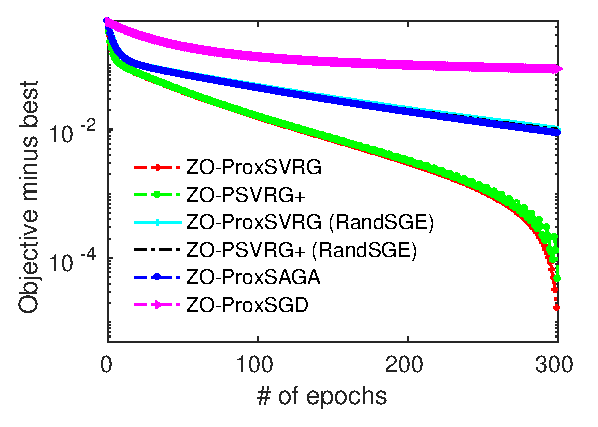
\includegraphics[width=0.3\linewidth]{Figures/binary/ijcnn1b50k1.eps}}%
\addtocounter{subfigure}{-4}
\subfigure{
\centering
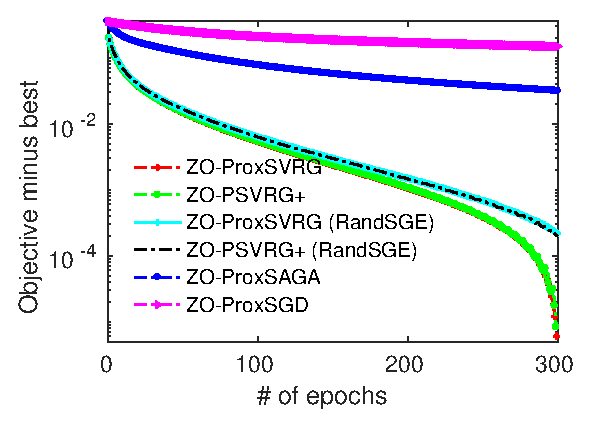
\includegraphics[width=0.3\linewidth]{Figures/binary/adultb50k1.eps}}%
\subfigure{
\centering
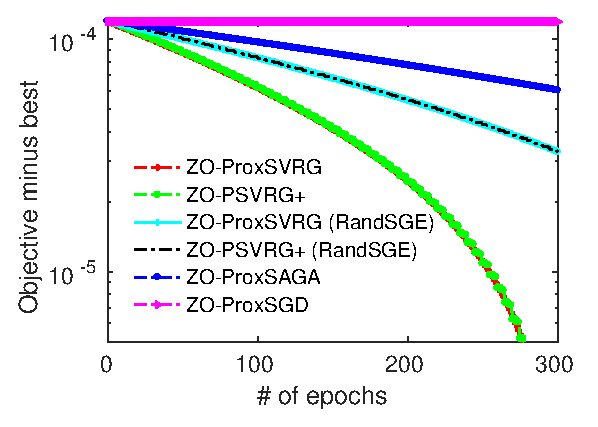
\includegraphics[width=0.3\linewidth]{Figures/binary/w8ab50k1.eps}}%
\subfigure{
\centering
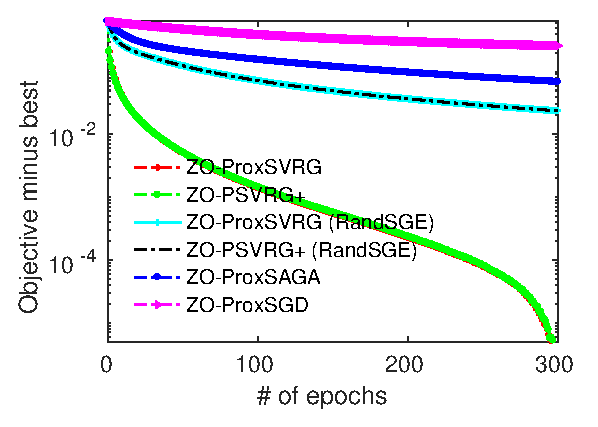
\includegraphics[width=0.3\linewidth]{Figures/binary/mnistb50k1.eps}}\\
\subfigure[ijcnn]{
\centering
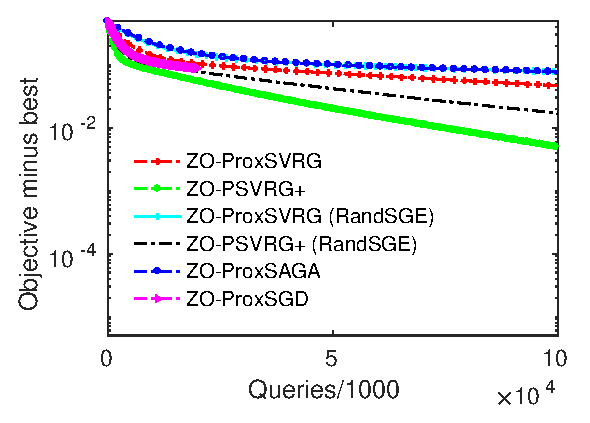
\includegraphics[width=0.3\linewidth]{Figures/binary/ijcnn1b50k2.eps}}%
\subfigure[comparison on covtype]{
\centering
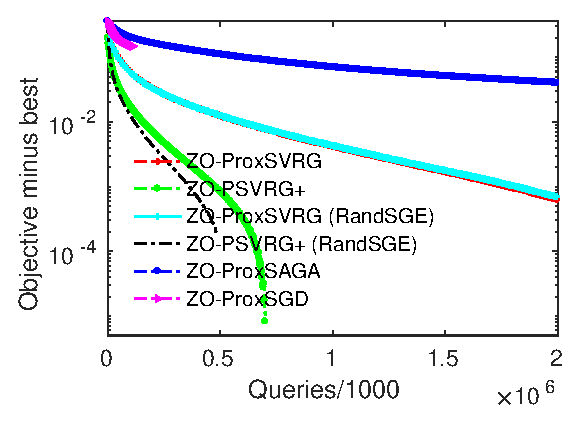
\includegraphics[width=0.3\linewidth]{Figures/binary/adultb50k2.eps}}%
\subfigure[w8a]{
\centering
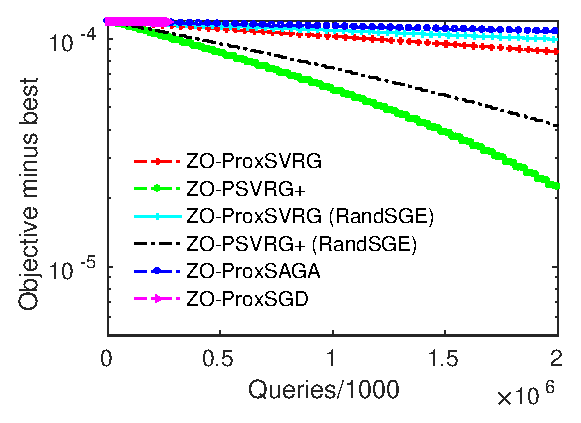
\includegraphics[width=0.3\linewidth]{Figures/binary/w8ab50k2.eps}}%
\subfigure[mnist]{
\centering
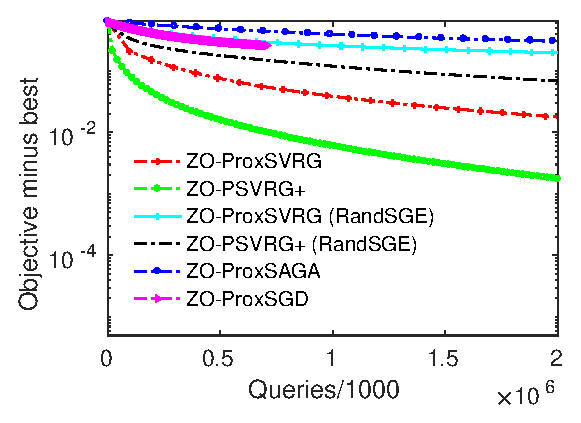
\includegraphics[width=0.3\linewidth]{Figures/binary/mnistb50k2.eps}}%
\setlength{\abovecaptionskip}{2pt}
\caption{Comparison of different zeroth-order algorithms for logistic regression loss residual $f(x) - f(x^*)$ versus the number of epochs (top) and ZO queries (bottom)}
\label{fig:algo_comp}
\end{figure*}


\subsection{Adversarial Attacks on Black-Box DNNs}

{\color{Brown}
Adversarial 
examples in image classification is related to designing unperceptive perturbations such that, by adding to the natural images, lead to misclassifying the target model. In the framework of zeroth-order attacks \cite{chen2017zoo,liu2018zeroth}, the model parameters are unexposed and obtaining its gradient is not feasible and only
the model evaluations are available. We can then consider the task of producing a universal adversarial
example with respect to $n$ natural images as an ZO optimization problem of the form \eqref{problem}.
{\color{Green}
More precisely, we apply the zeroth-order algorithms to obtain a global adversarial perturbation $x\in\R^d$ that could mislead the classifier on samples $\{a_i \in \R^d, y_i\in\mathbb{N} \}_{i=1}^n$. This problem can be specified as the following elastic-net attacks to black-box DNNs problem:
\begin{equation}\label{mnist-attack-loss}
\begin{split}
\min_{x\in\R^d} \frac{1}{n} \sum_{i=1}^n& \max\{F_{y_i}(a_i^{adv}) - \max_{j\neq y_i}F_j(a_i^{adv}),0\} + c\norm{a_i^{adv} - a_i}^2 \\
&+ \lambda_1 \norm{x}_{1} + \lambda_2 \norm{x}^{2}
\end{split}
\end{equation}
where $a_i^{adv} = 0.5\tanh(\tanh^{-1}(2a_i)+x)$ and $\lambda_1$ and $\lambda_2$ are nonnegative parameters to harmonize attack success rate, distortion and sparsity. Here $F(a) = \left[F_1(a),\ldots,F_K(a)\right]\in [0, 1]^K$ describes a trained DNN{\footnote{https://github.com/carlini/nn$\underline{~~}$robust$\underline{~~}$attacks}} for the MNIST handwritten digit classification, where $F_i(a)$ returns the prediction score of $i$-th class. {\color{Brown} The parameter $c$ in \eqref{mnist-attack-loss} compensate the rate of adversarial success and the distortion of adversarial examples. In our experiment, we set the regularization parameter  $c = 0.2$. In addition, we set {\color{red} $\lambda_1 = 10^{-5}$} and {\color{red} $\lambda_2 = 10^{-5}$} in the experiments.  }

}
We perfrom two experiments by choosing $n = 10$ and $n=100$ images from the same class, and set the minibatch sizes, respectively $b=5$ and $b = 30$. The stepsizes are selected {\color{red} $30/d$} and {\color{red} $30/d$} respectively for ZO-PSVRG+  and ZO-PSVRG+ (RandSGE), where $d = 28 \times 28$ is the image dimension. The stepsize $\eta$ for other algorithms are selected according to Table \ref{table-compare}. We select the batch size $\mathcal{B} = \lfloor{\frac{n}{2}}\rfloor$ for ZO-PSVRG+.
{\color{Green}

}
}
{\color{Melon}
Figure \ref{attack-fig} shows
the performance of different ZO algorithms considered in this paper. Our two algorithms ZO-PSVRG+ (RandSGE) and ZO-ProxSVRG (under our improved analysis) show better performance
both in convergence rate (iteration complexity) and function query complexity than ZO-ProxSGD
and ZO-ProxSAGA. The performance of ZO-PSVRG+ (CoordSGE) algorithm degrades due to large number of function queries for CoordSGE and the variance inherited by $\mathcal{B} \neq n$. 
ZO-PSVRG+ (RandSGE) shows faster convergence in the initial optimization stage, and more importantly, has much lower function query complexity, which is largely
due to efficient ZO queries for computing mix gradient \eqref{zo-grad-fo-rand} and  the $O(\frac{1}{\sqrt{d}})$-level stepsize required by ZO-PSVRG+ (RandSGE).
}
\begin{figure*}[htbp]\label{attack-fig}
\subfigure[Loss vs iterations: $n = 10$]{
\centering
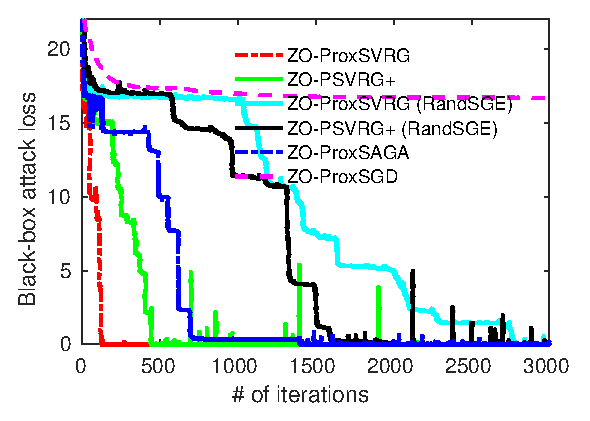
\includegraphics[width=0.3\linewidth]{Figures/attack/figiter.eps}}%
\subfigure [Loss vs queries: $n = 10$]{
\centering
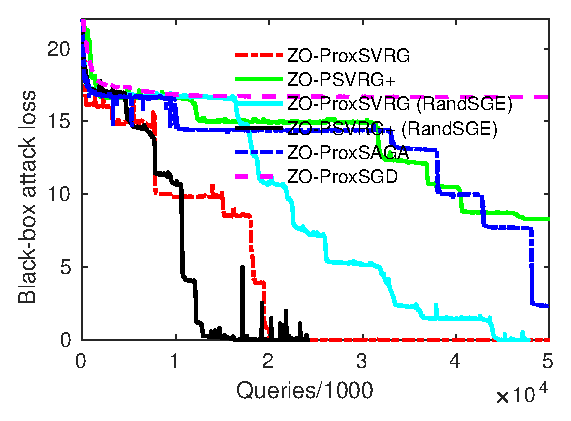
\includegraphics[width=0.3\linewidth]{Figures/attack/figquery.eps}}%
\setlength{\abovecaptionskip}{2pt}
\caption{Comparison of different zeroth-order algorithms for generating black-box adversarial examples from a black-box DNN}
\end{figure*}
{\color{Brown}
ZO-ProxSAGA and ZO-PSVRG+ (CoordSGE) exhibit relatively similar convergence behavior. Furthermore, the convergence performance of ZO-ProxSGD is poor compared to other algorithms due to using variance reduced algorithms. 
}

\section{Appendix}
In this section, we present the complete proofs of the above lemmas and theorems. In the beginning, we give some useful properties of CoordSGE and RandSGE, respectively.
\begin{lemma}[\cite{liu2018zeroth}]\label{CooSGE}
Suppose that the function $f(x)$ is $L$-smooth. Let $\hat{\nabla} f(x)$ denote the estimated gradient defined by CoordSGE. Define $f_{\mu} = \E_{u\sim U[-\mu, \mu]} f(x+ue_j)$, where $U[-\mu,\mu]$ denotes the uniform distribution on the interval $[-\mu, \mu]$. Then for any $x \in \R^d$ we have 
\begin{enumerate}
\item $f_{\mu}$ is $L$-smooth, and 
$\hat{\nabla} f(x) = \sum_{j=1}^d \frac{\partial f_{\mu}(x)}{\partial x_j}e_j$.

\item $\abs{f_{\mu}(x) - f(x)} \leq \frac{L\mu^2}{2}$ and $\abs{\frac{\partial f_{\mu}(x)}{\partial x_j}} \leq \frac{L\mu^2}{2}$.
 
\item $\norm{\hat{\nabla} f(x) - {\nabla} f(x)} ^2 \leq \frac{L^2 d^2 \mu^2}{4}$.
\end{enumerate}  
\end{lemma}
\begin{theorem}\label{SGERand-approx}
Assume that the function $f(x)$ is $L$-smooth. Let $\hat{\nabla}_r f(x)$ denote the estimated gradient defined by RandSGE. Define $f_{\mu} = \E_{u\sim U_S}[f(x+\mu u)]$, where $U$ is uniform distribution over a $d$-dimensional unit ball $S$. Then, we have 
\begin{enumerate}
\item For any $x \in \R^d$, $\nabla f_{\mu}(x) = \E_u[\hat{\nabla}_r f(x,u)]$.\\
\item $\abs{f_{\mu}(x) - f(x)} \leq \frac{\mu^2 L}{2}$ and 
$\norm{f_{\mu}(x) - f(x)} \leq \frac{\mu L d}{2}$ for any $x \in \R^d$.\\
\item $\E_{u}\norm{\hat{\nabla}_r f(x,u) - \hat{\nabla}_r f(y,u)}^2 \leq 3dL^2\norm{x-y}^2 + \frac{3L^2d^2\mu^2}{2}$.
\end{enumerate}
\end{theorem}
\begin{proof}
The proof of items $1$ and $2$ can be found in \cite{gao2018information}. Item 3 is due to Lemma 5 in \cite{ji2019improved}.  
\end{proof}
\begin{lemma}\label{lemma1}
For a given $x \in \R^d$, let $\overline{x} = \Po_{\eta h}(x-\eta v)$, then we have for all $w\in \R^d$
\begin{equation}\label{eq10}
\begin{split}
F(\overline{x}) \leq F(w) &+ \Iprod{\nabla f(x)-v}{\overline{x}-w}-\frac{1}{\eta} \Iprod{\overline{x}-x}{\overline{x}-w}\\
&+\frac{L}{2}\norm{\overline{x}-x}^2+\frac{L}{2}\norm{w-x}^2 
\end{split}
\end{equation}
\end{lemma}
\begin{proof}
First, we recall the proximal operator 
\begin{equation}\label{eq11}
\Po_{\eta h}(x-\eta v) := \text{arg}\,\,\min_{y\in\R^d}\left(h(y)+\frac{1}{2\eta}\norm{y-x}^2+\Iprod{v}{y}\right)
\end{equation}
For the nonsmooth function $h(x)$, for all $w\in\R^d$ we have 
\begin{equation}\label{eq12}
\begin{split}
h(\overline{x}) &\leq h(w) + \Iprod{p}{\overline{x}-w}\\
&= h(w) - \Iprod{v+\frac{1}{\eta}(\overline{x}-x)}{\overline{x}-w}
\end{split}
\end{equation}
where $p\in \partial h(\overline{x})$ such that $p+\frac{1}{\eta}(\overline{x}-x)+v = 0$ according to the optimality condition of \eqref{eq11}, and \eqref{eq12} due to the convexity of $h$. In addition, since since $f(x)$ is $L$-Lipschitz continuous, we have
\begin{equation}\label{eq14}
f(\overline{x}) \leq f(x)+\Iprod{\nabla f(x)}{\overline{x}-x}+\frac{L}{2}\norm{\overline{x}-x}^2
\end{equation}
and
\begin{equation}\label{eq15}
f(x) \leq f(w)+\Iprod{\nabla f(x)}{x-w}+\frac{L}{2}\norm{w-x}^2
\end{equation}
 This lemma is obtained by adding \eqref{eq12}, \eqref{eq14}, \eqref{eq15}, and using $F(x) = f(x)+h(x)$. 
\end{proof}
\begin{lemma}\label{lemm-est-grad}
Let  $x_{t}^s= \Po_{\eta h}(x_{t-1}^s - \eta \hat{v}_{t-1}^s)$ and $\overline{x}_{t}^s$ be the proximal projection using full true gradient, i.e., $\overline{x}_{t}^s= \Po_{\eta h}(x_{t-1}^s - \eta \nabla f(x_{t-1}^s))$. Then the following inequality holds
\[
\Iprod{\nabla f(x_{t-1}^s) -\hat{v}_{t-1}^s)}{x_t^s -\overline{x}_t^s} \leq \eta\norm{\nabla f(x_{t-1}^s)-\hat{v}_{t-1}^s}^2
\]
\end{lemma}
\begin{proof}
Based on inequality \eqref{eq12} we obtain
\begin{align}
h(x_t^s)&\leq h(\overline{x}_t^s) - \Iprod{\hat{v}_{t-1}^s+\frac{1}{\eta}(x_t^s-x_{t-1}^s)}{x_t^s-\overline{x}_t^s}\label{lemm-est-grad-1}
\end{align}
\begin{align}
h(\overline{x}_t^s)&\leq h({x}_t^s) - \Iprod{\nabla f(x_{t-1}^s)+\frac{1}{\eta}(\overline{x}_t^s-x_{t-1}^s)}{\overline{x}_t^s-x_t^s}\label{lemm-est-grad-2}
\end{align}
By summing \eqref{lemm-est-grad-1} and \eqref{lemm-est-grad-2}, we have 
\begin{align}
\frac{1}{\eta}\Iprod{x_t^s -\overline{x}_t^s}{x_t^s -\overline{x}_t^s} &\leq \Iprod{\nabla f(x_{t-1}^s) -\hat{v}_{t-1}^s}{x_t^s -\overline{x}_t^s}\notag\\
\frac{1}{\eta}\norm{x_t^s -\overline{x}_t^s}^2 &\leq \norm{\nabla f(x_{t-1}^s) -\hat{v}_{t-1}^s}\norm{x_t^s -\overline{x}_t^s}\label{lemm-est-grad-3}
\end{align}
where \eqref{lemm-est-grad-3} holds by Cauchy-Schwarz inequality. 
Thus, we obtain
\begin{align}
\norm{x_t^s -\overline{x}_t^s} &\leq \eta\norm{\nabla f(x_{t-1}^s) -\hat{v}_{t-1}^s}\label{lemm-est-grad-4}
\end{align}
Now the proof is complete using Cauchy-Schwarz inequality and \eqref{lemm-est-grad-4}.
\end{proof}


\bibliographystyle{plainnat}
\bibliography{GTA}
\end{document}

